\chapter{Results}
\label{chap:chapter-4}


\section{V1}\label{sec:v1_results}

\begin{figure}
    \centering
    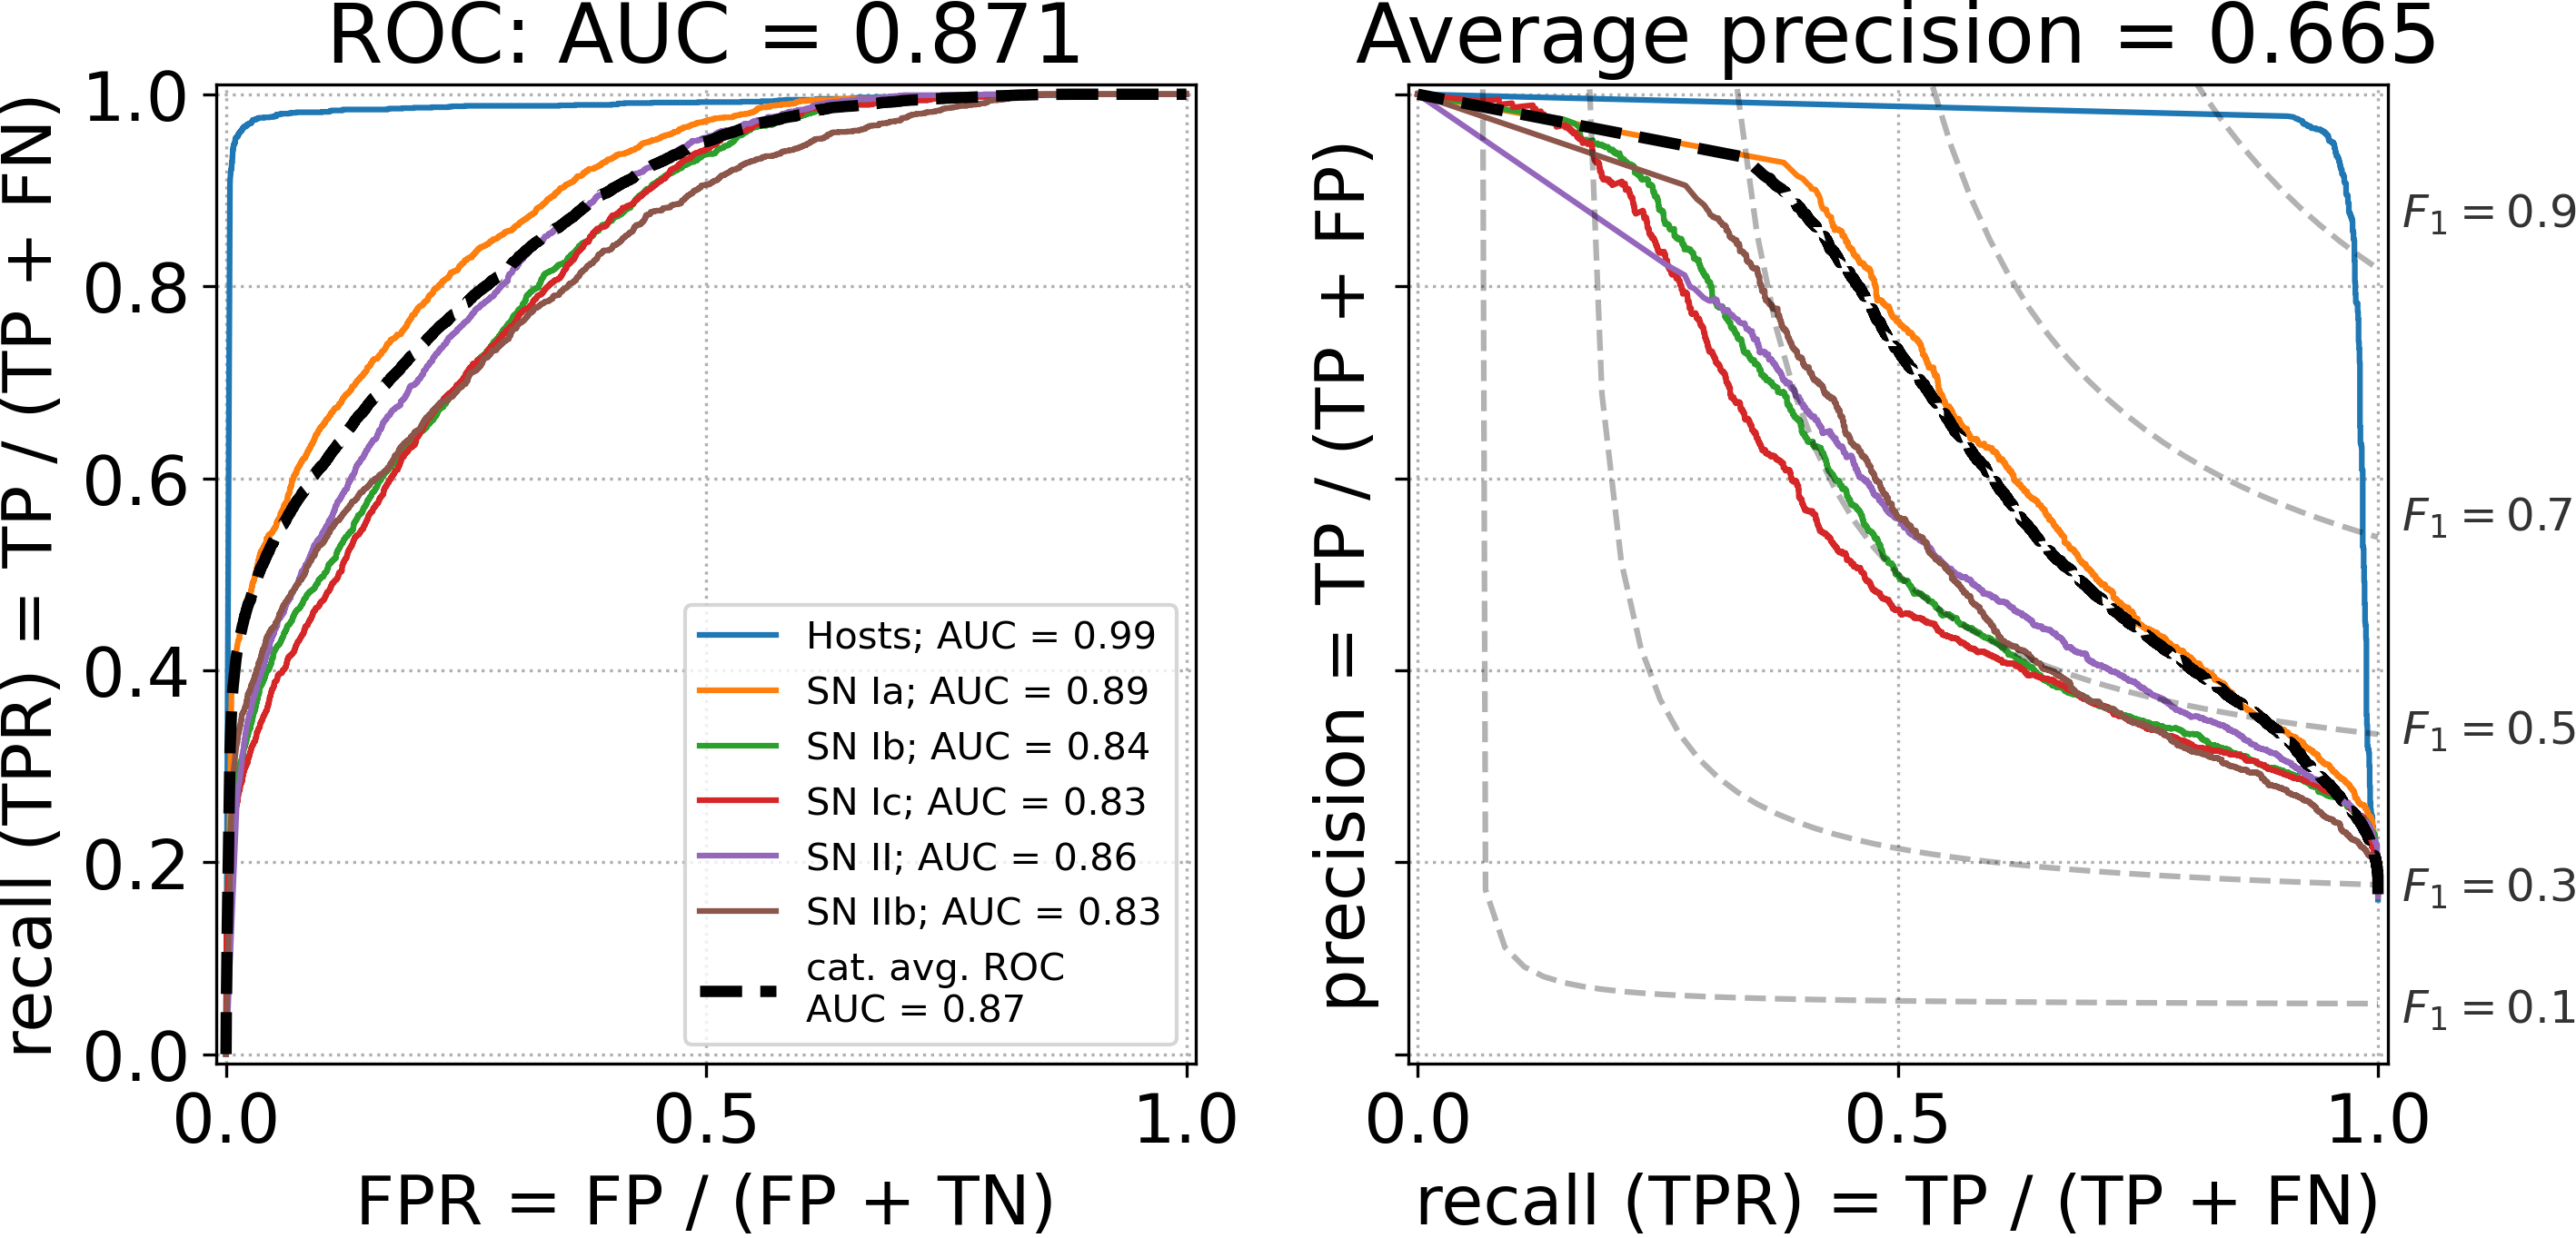
\includegraphics[height=4.3cm]{figures/v1_real/vit_model_V1_original_redorocfulle_e31.png}
    \quad
    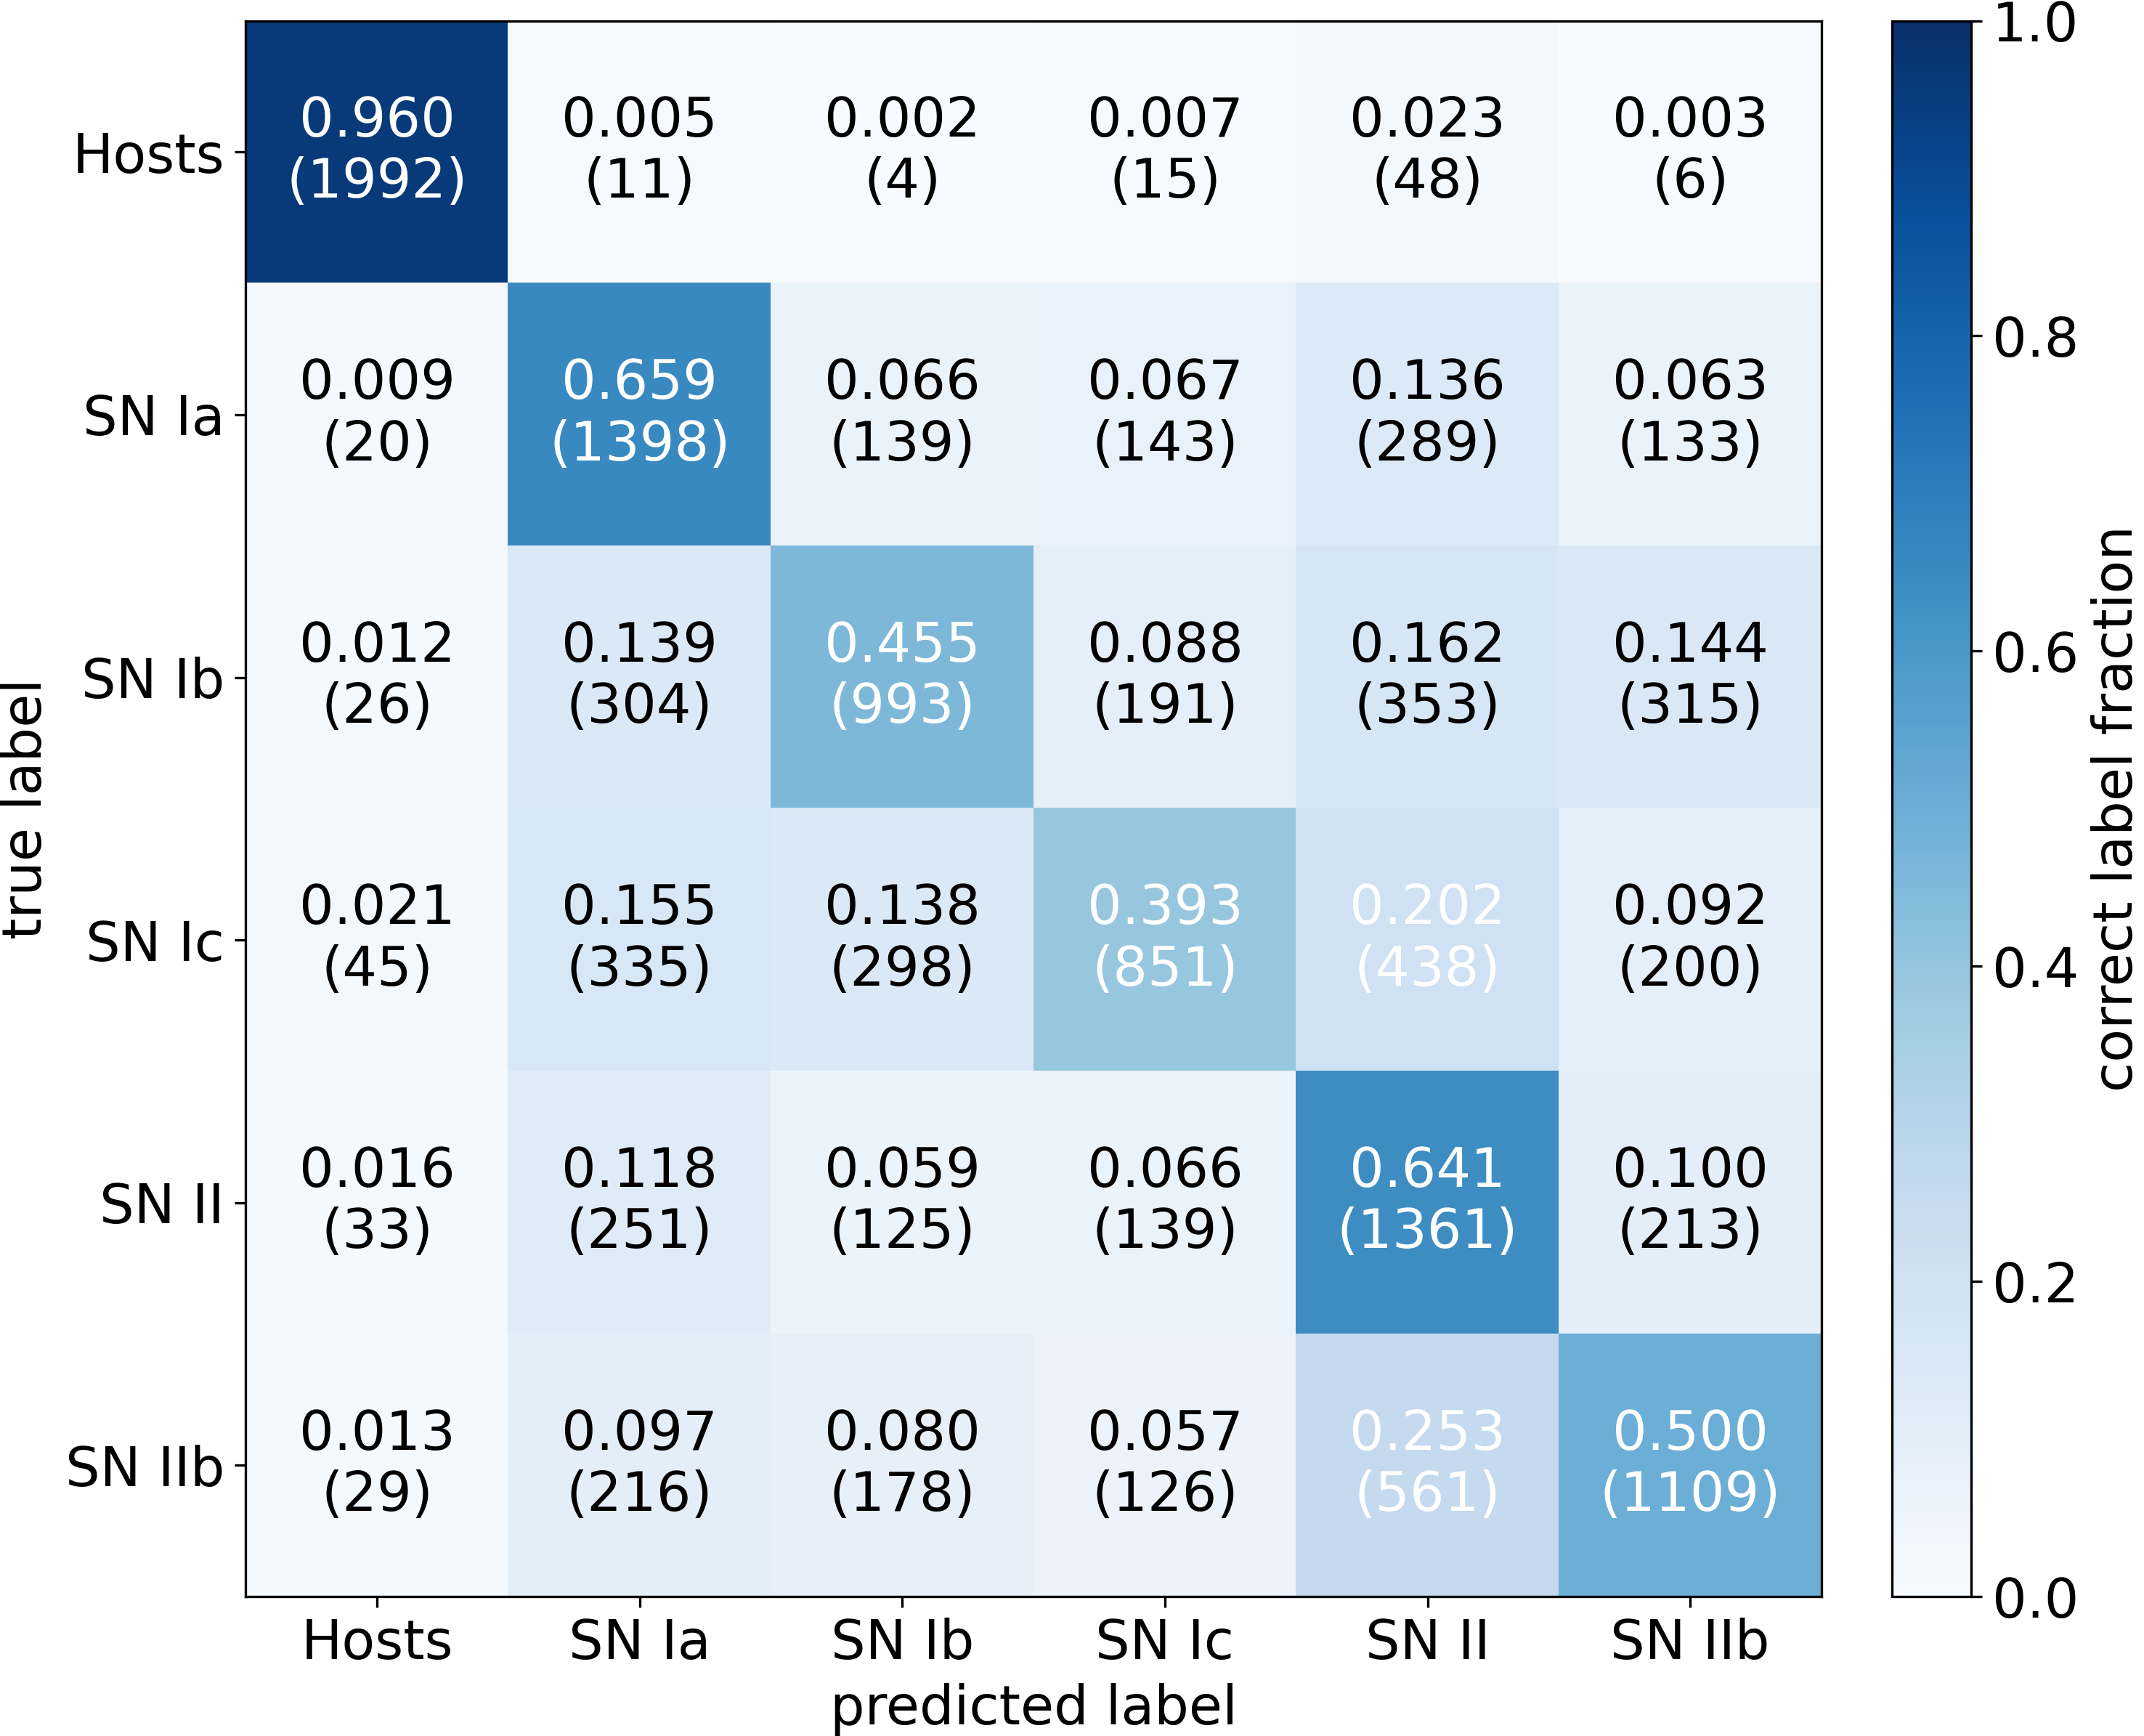
\includegraphics[height=4.3cm]{figures/v1_real/vit_model_V1_original_redocmfull_e31.png}
    \caption{Spectral ViT V1 Diagnostics: ROC Curve (left) and Confusion Matrix (right)\label{fig:v1_qual}}
\end{figure}

\begin{figure}
    \centering
    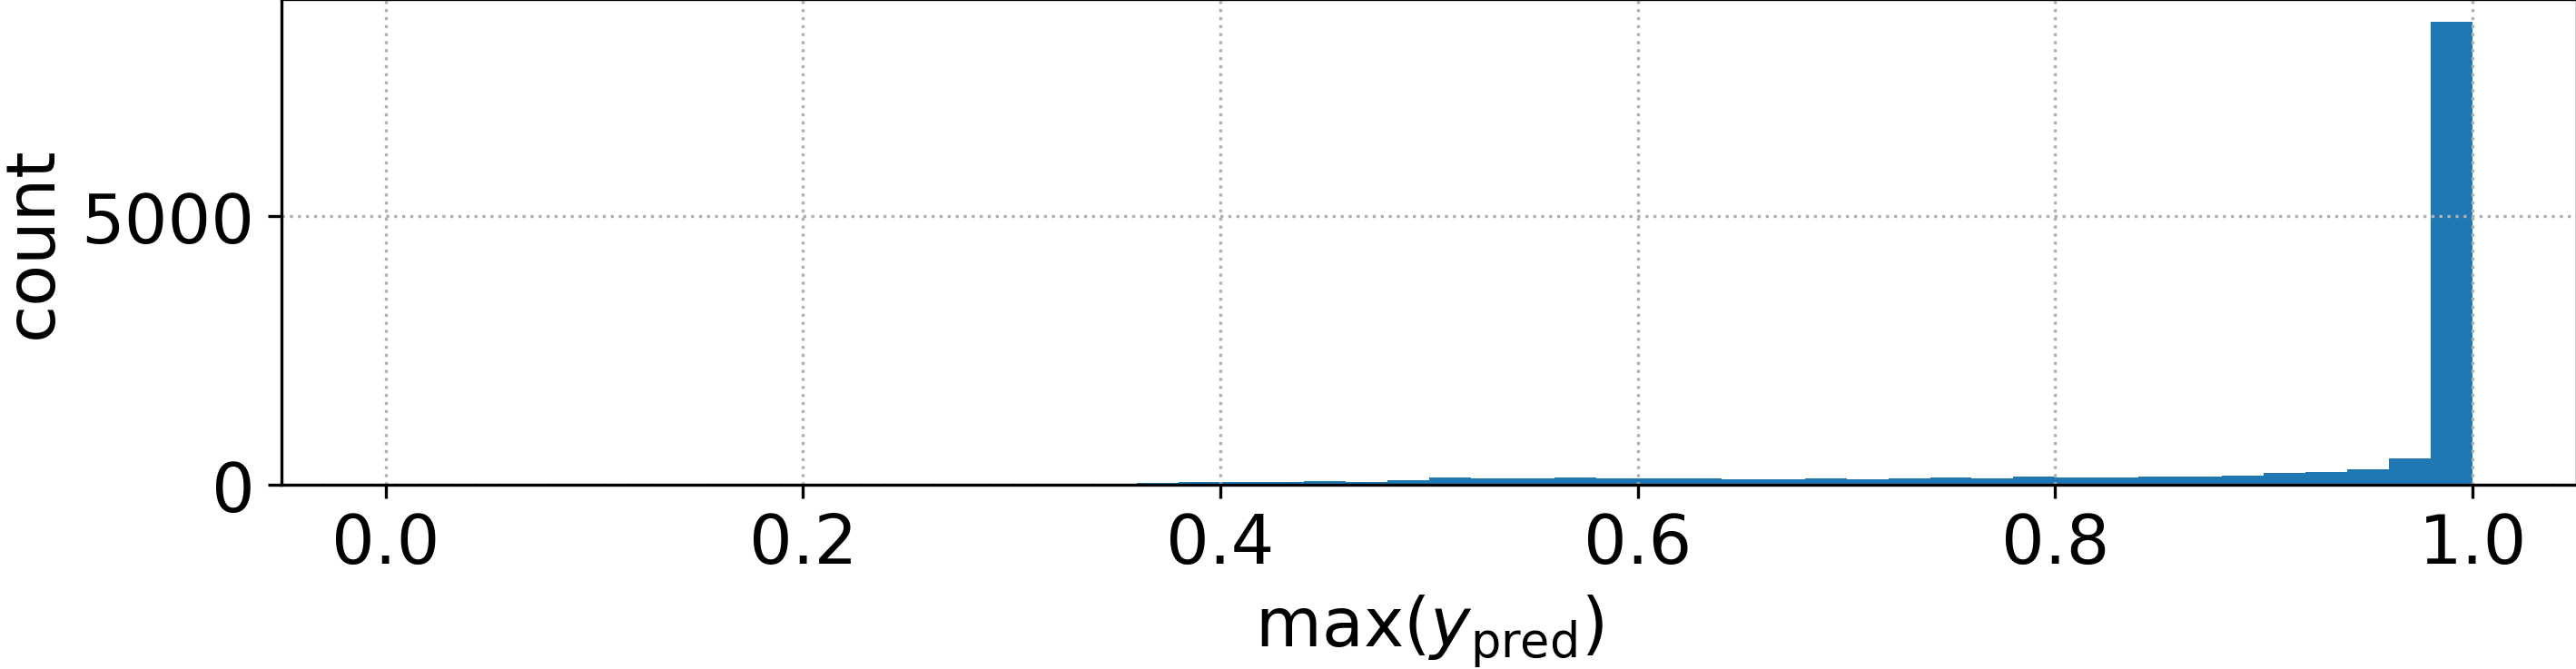
\includegraphics[width=0.6\textwidth]{figures/v1_real/vit_model_V1_original_redomax_ypred_binary_31.png}
    \caption{Max value of the output vector from the Spectral ViT V1.\label{fig:v1_max}}
\end{figure}



\begin{figure}
    \centering
    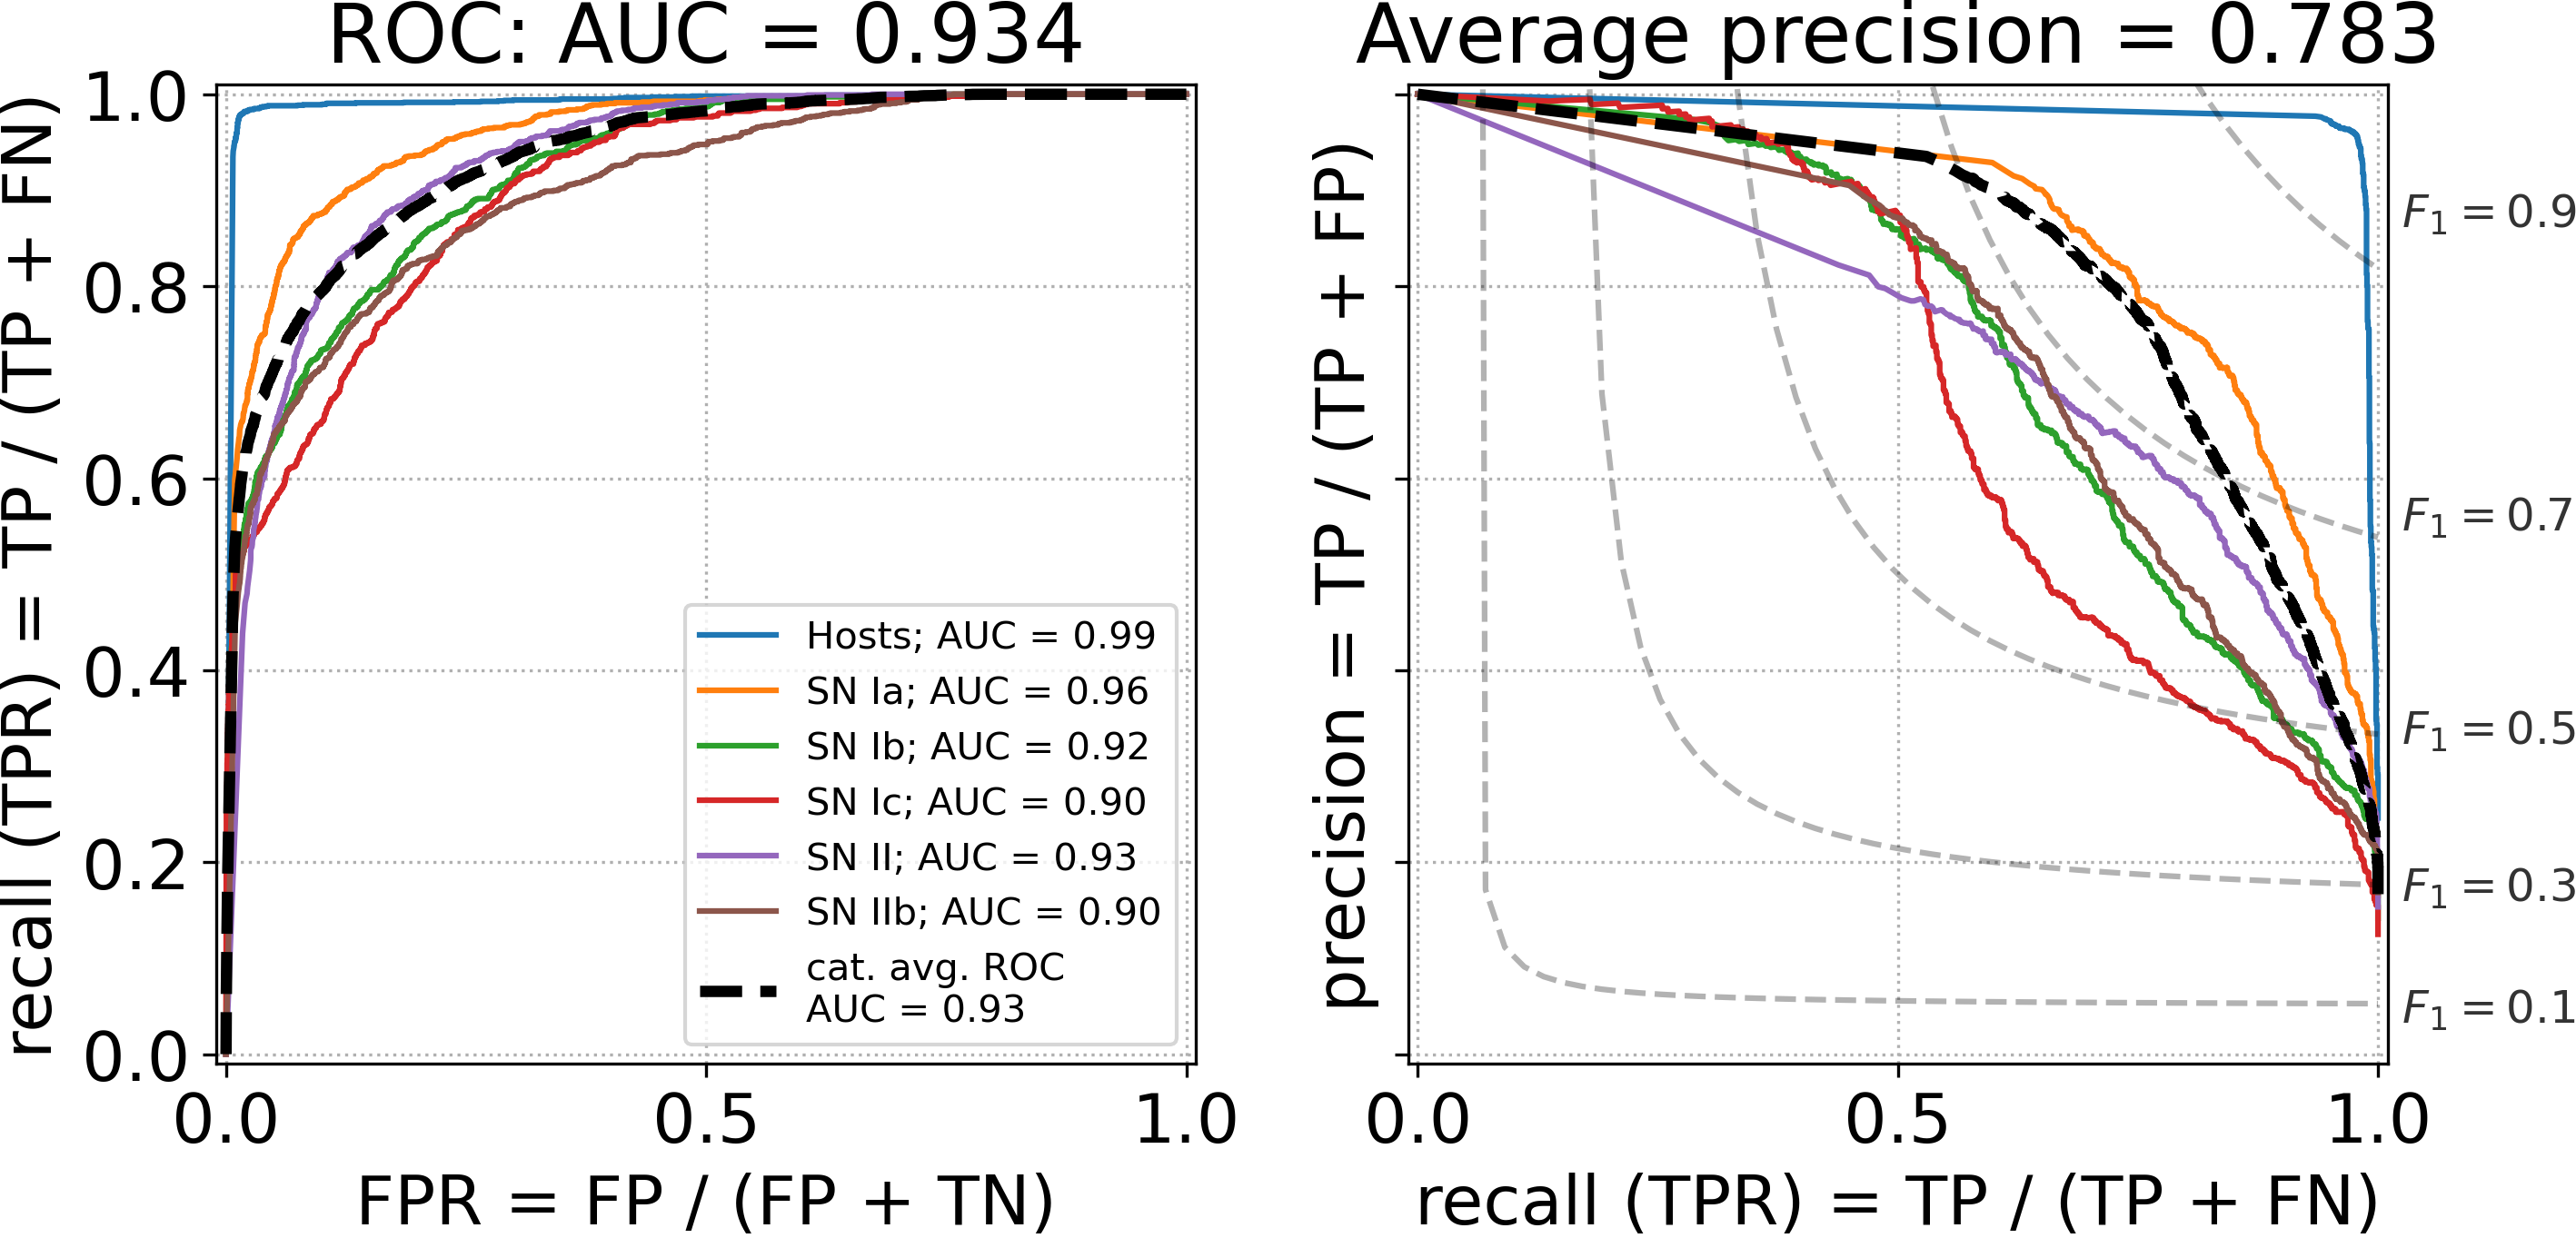
\includegraphics[height=4.3cm]{figures/v1_real/vit_model_V1_original_redoroc99_e31.png}
    \quad
    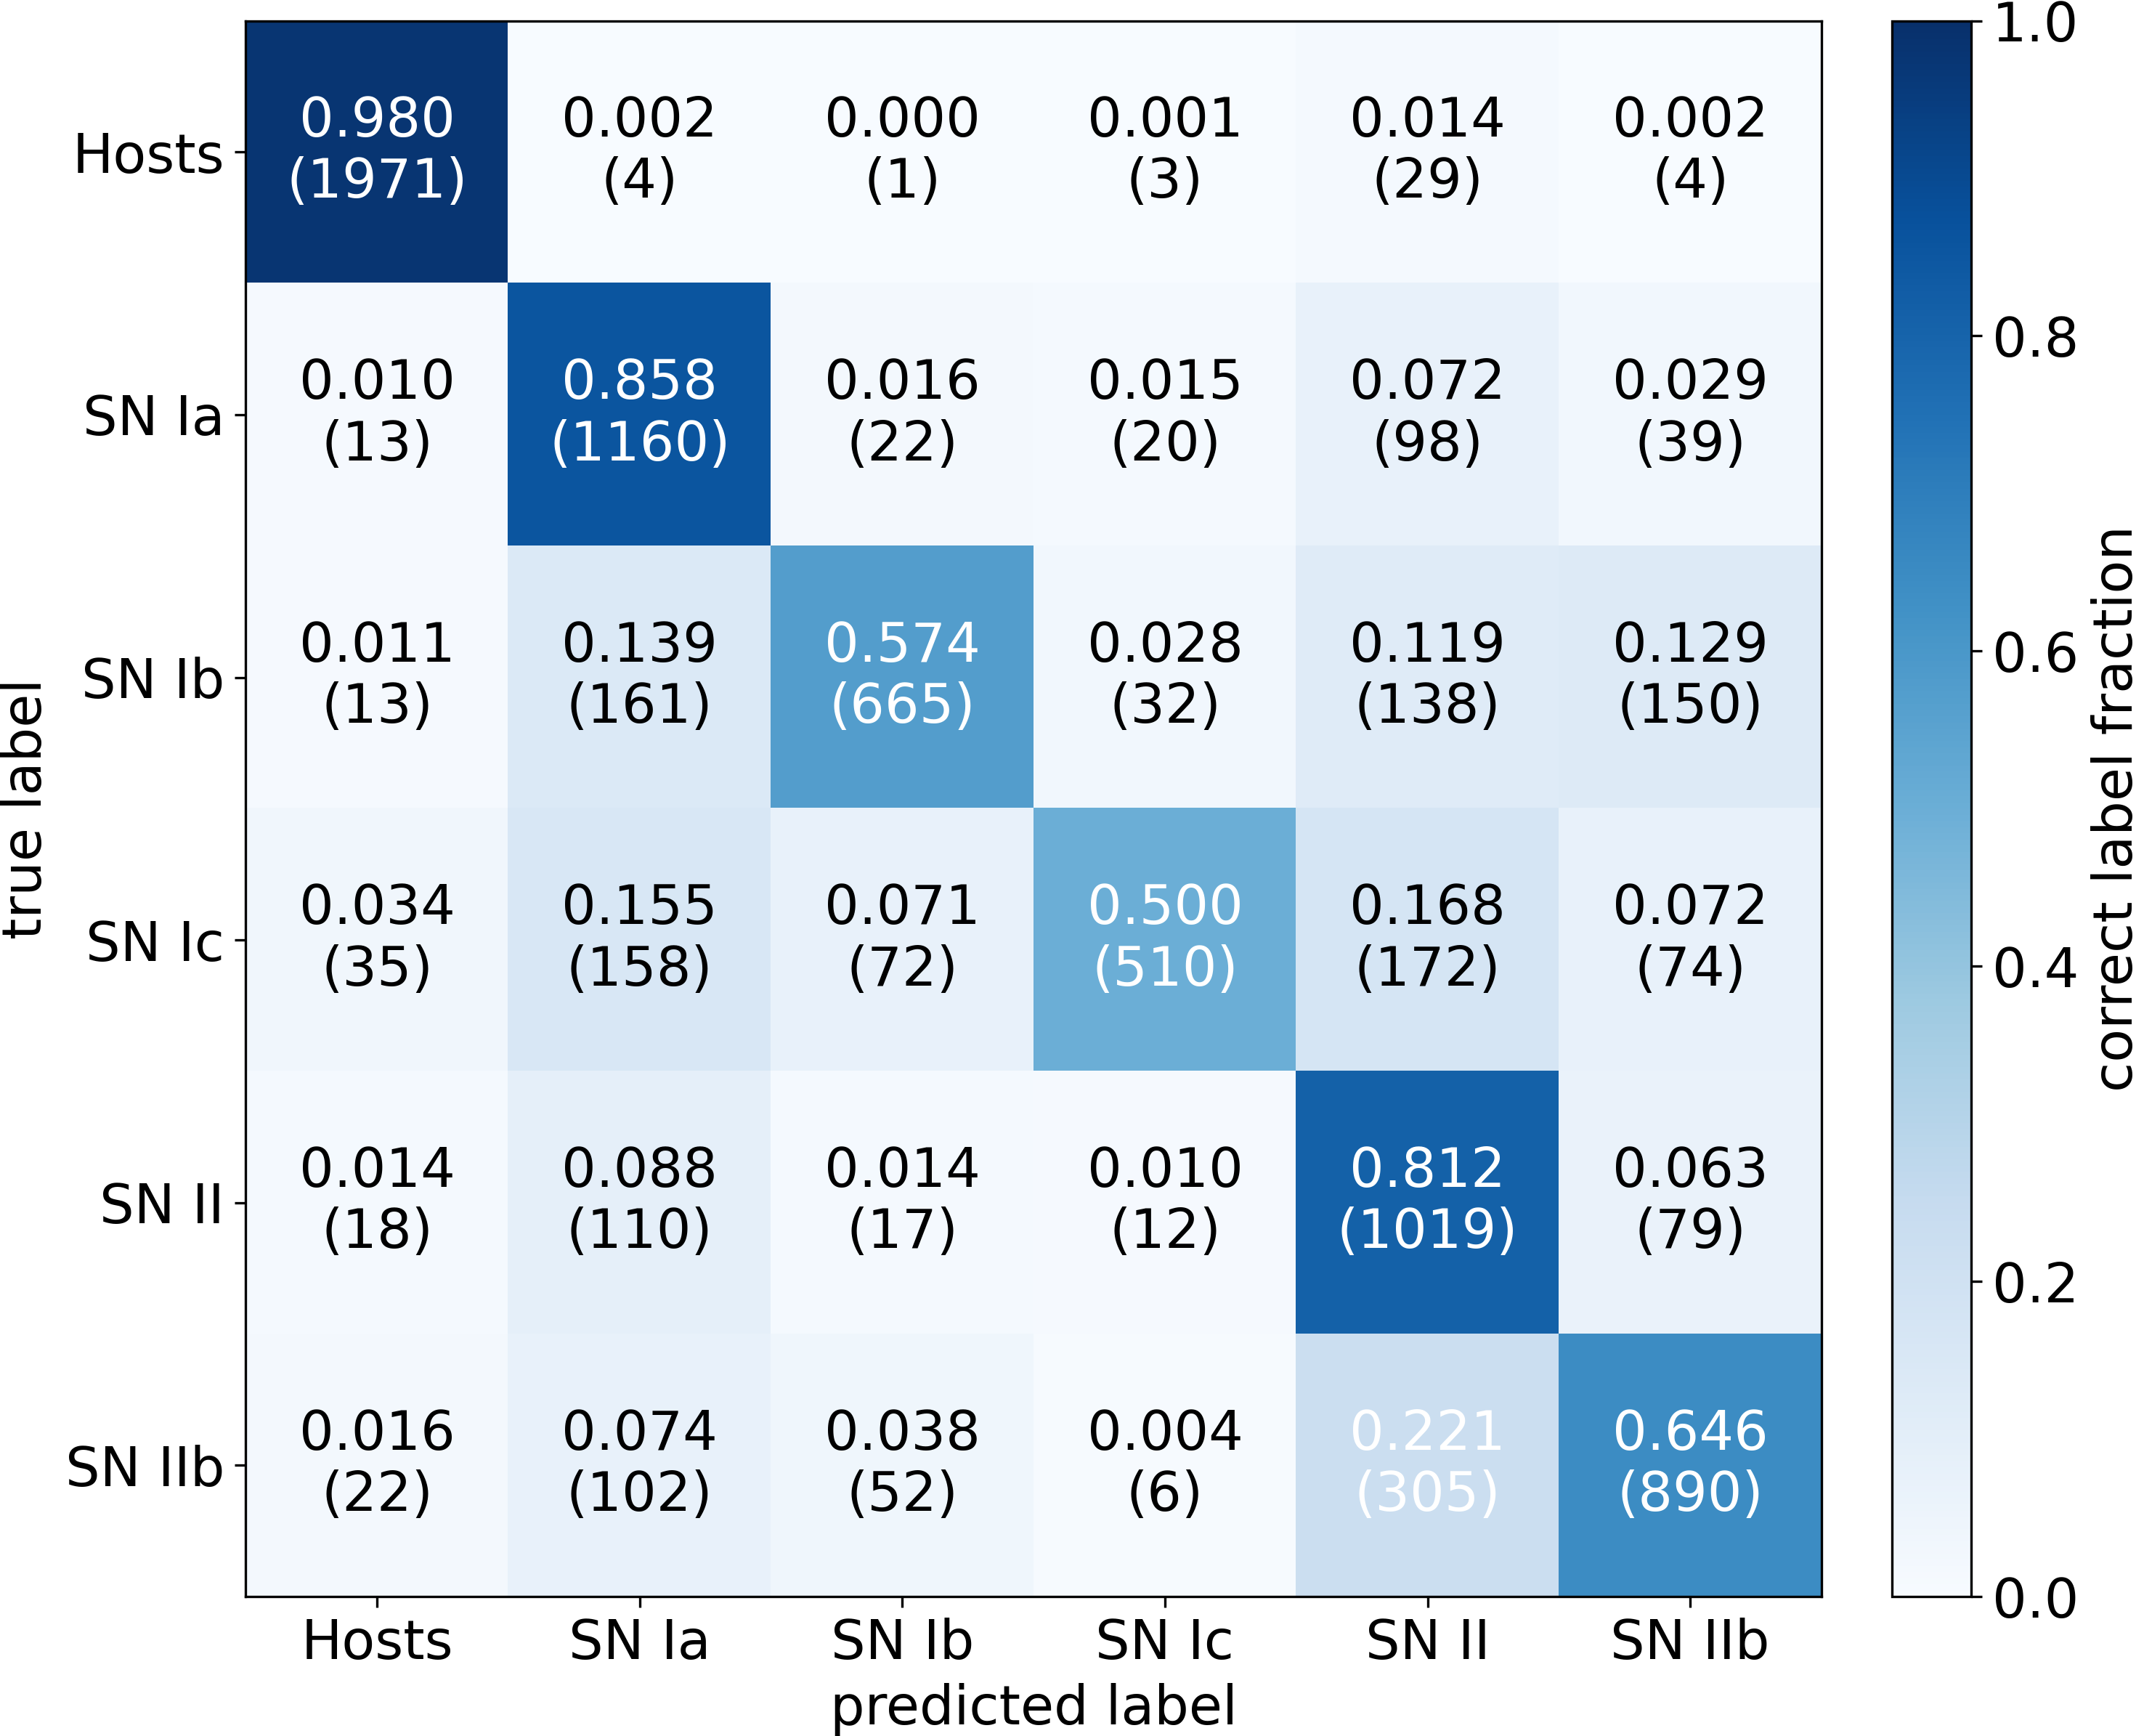
\includegraphics[height=4.3cm]{figures/v1_real/vit_model_V1_original_redocm99_e31.png}
    \caption{Spectral ViT V1 Diagnostics: ROC Curve (left) and Confusion Matrix (right) with a 99\% confidence
    cut \label{fig:v1_99_qual}}
\end{figure}


\begin{figure}
    \centering
    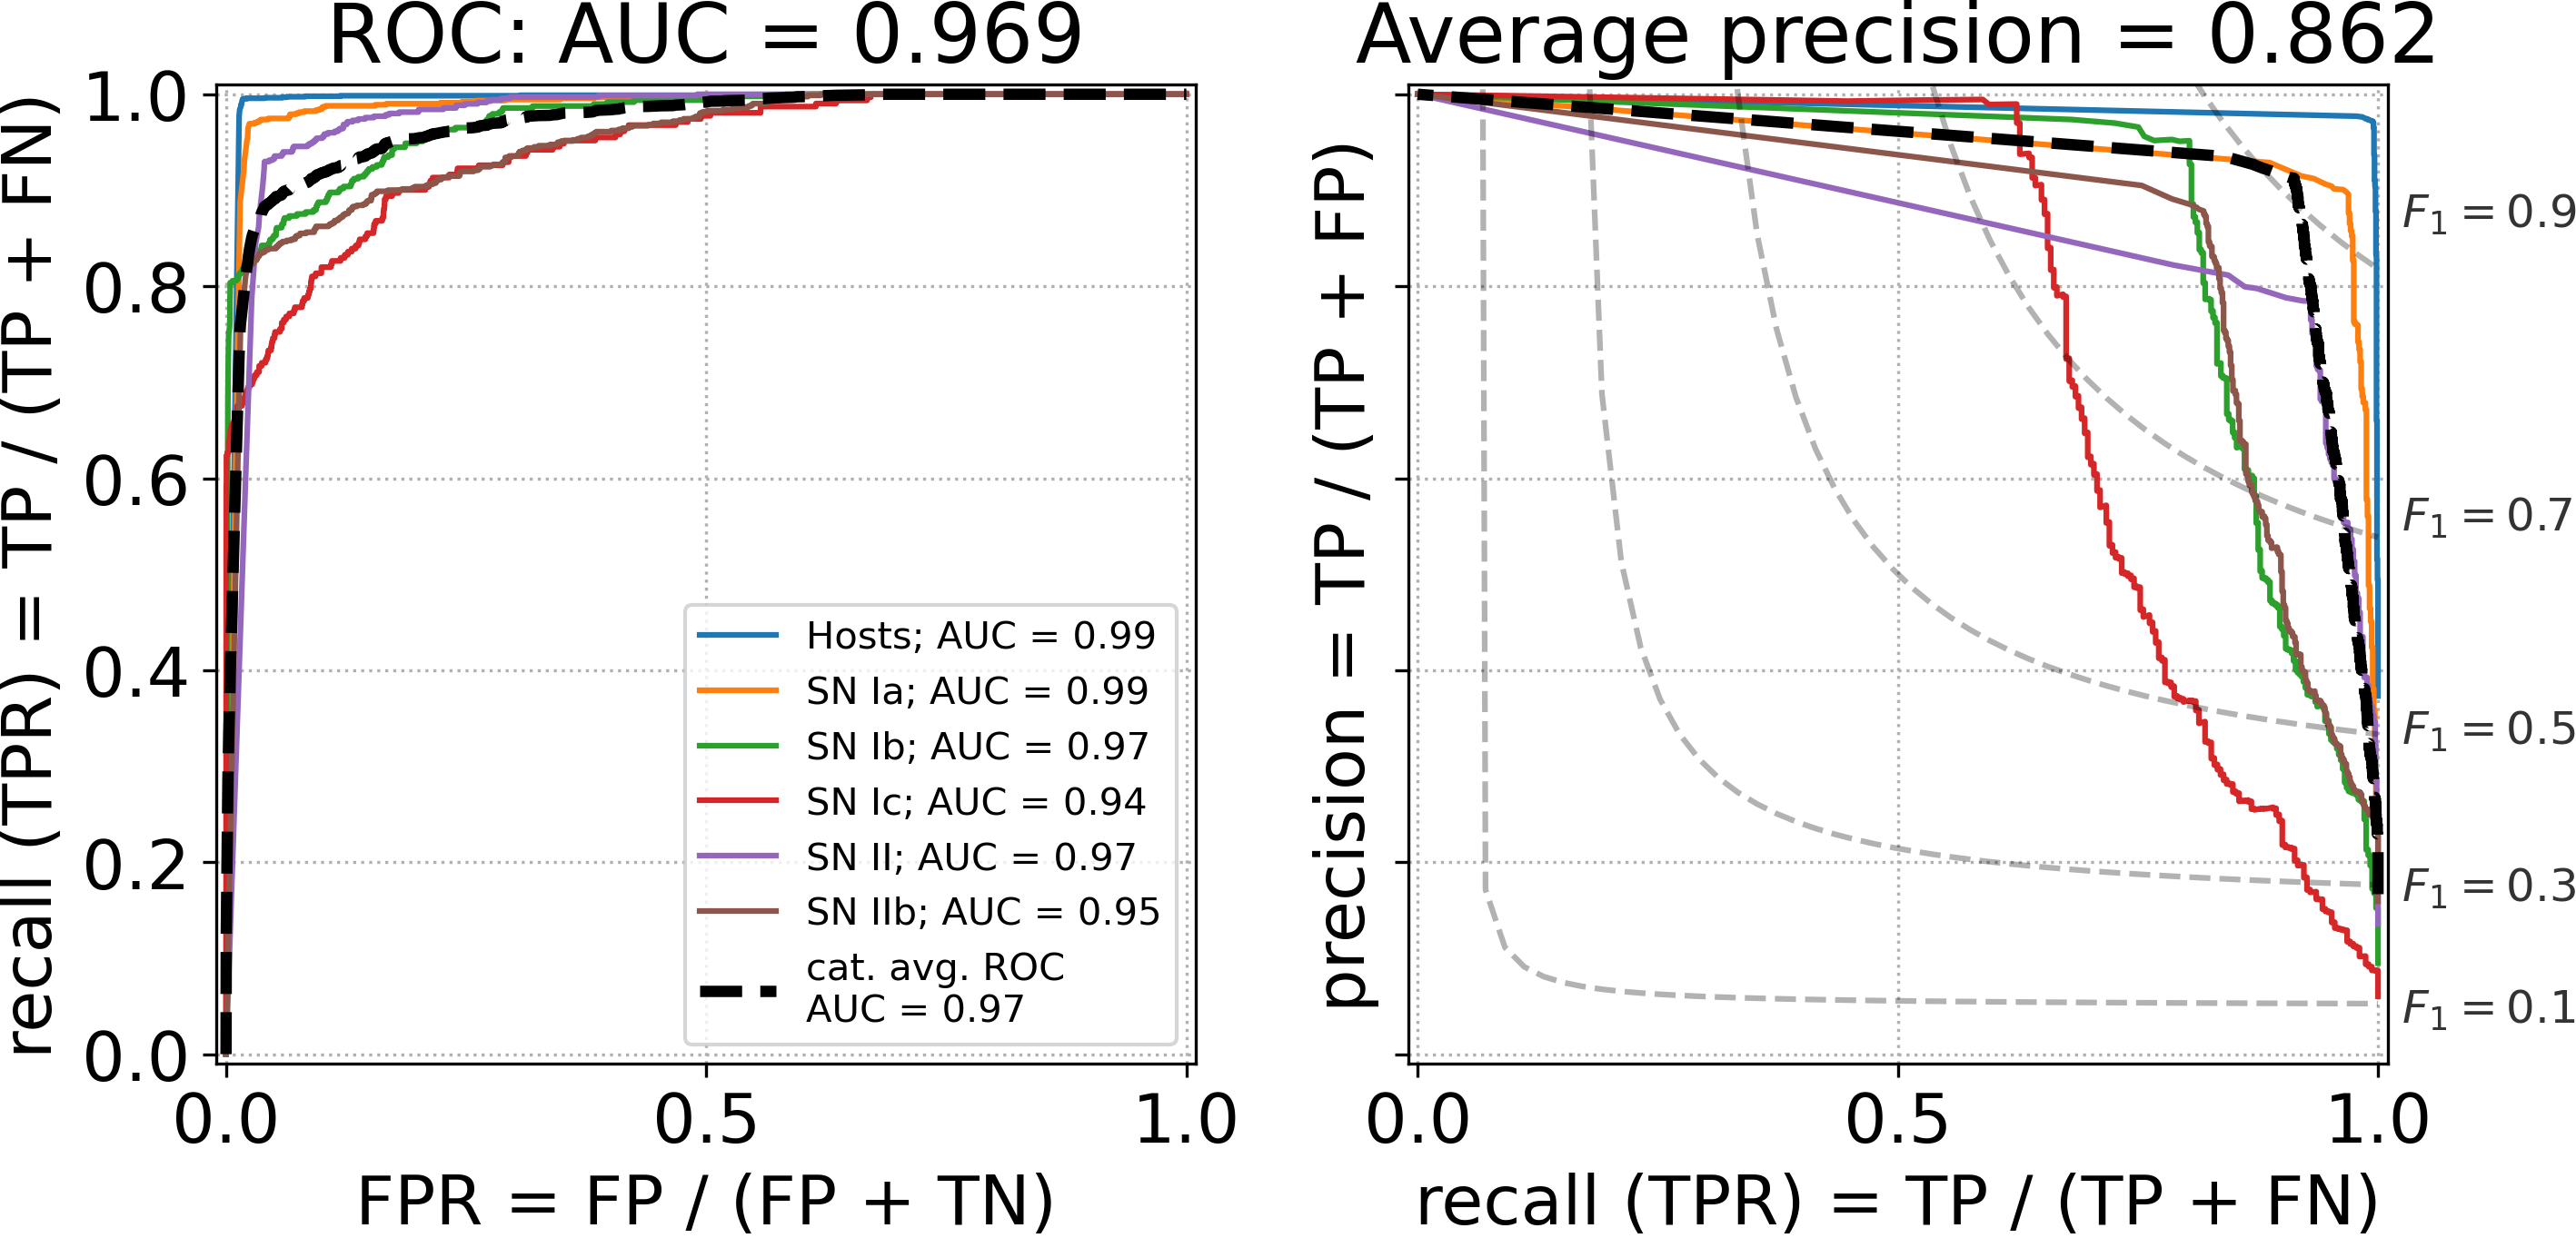
\includegraphics[height=4.3cm]{figures/v1_real/vit_model_V1_original_redoroc999999_e31.png}
    \quad
    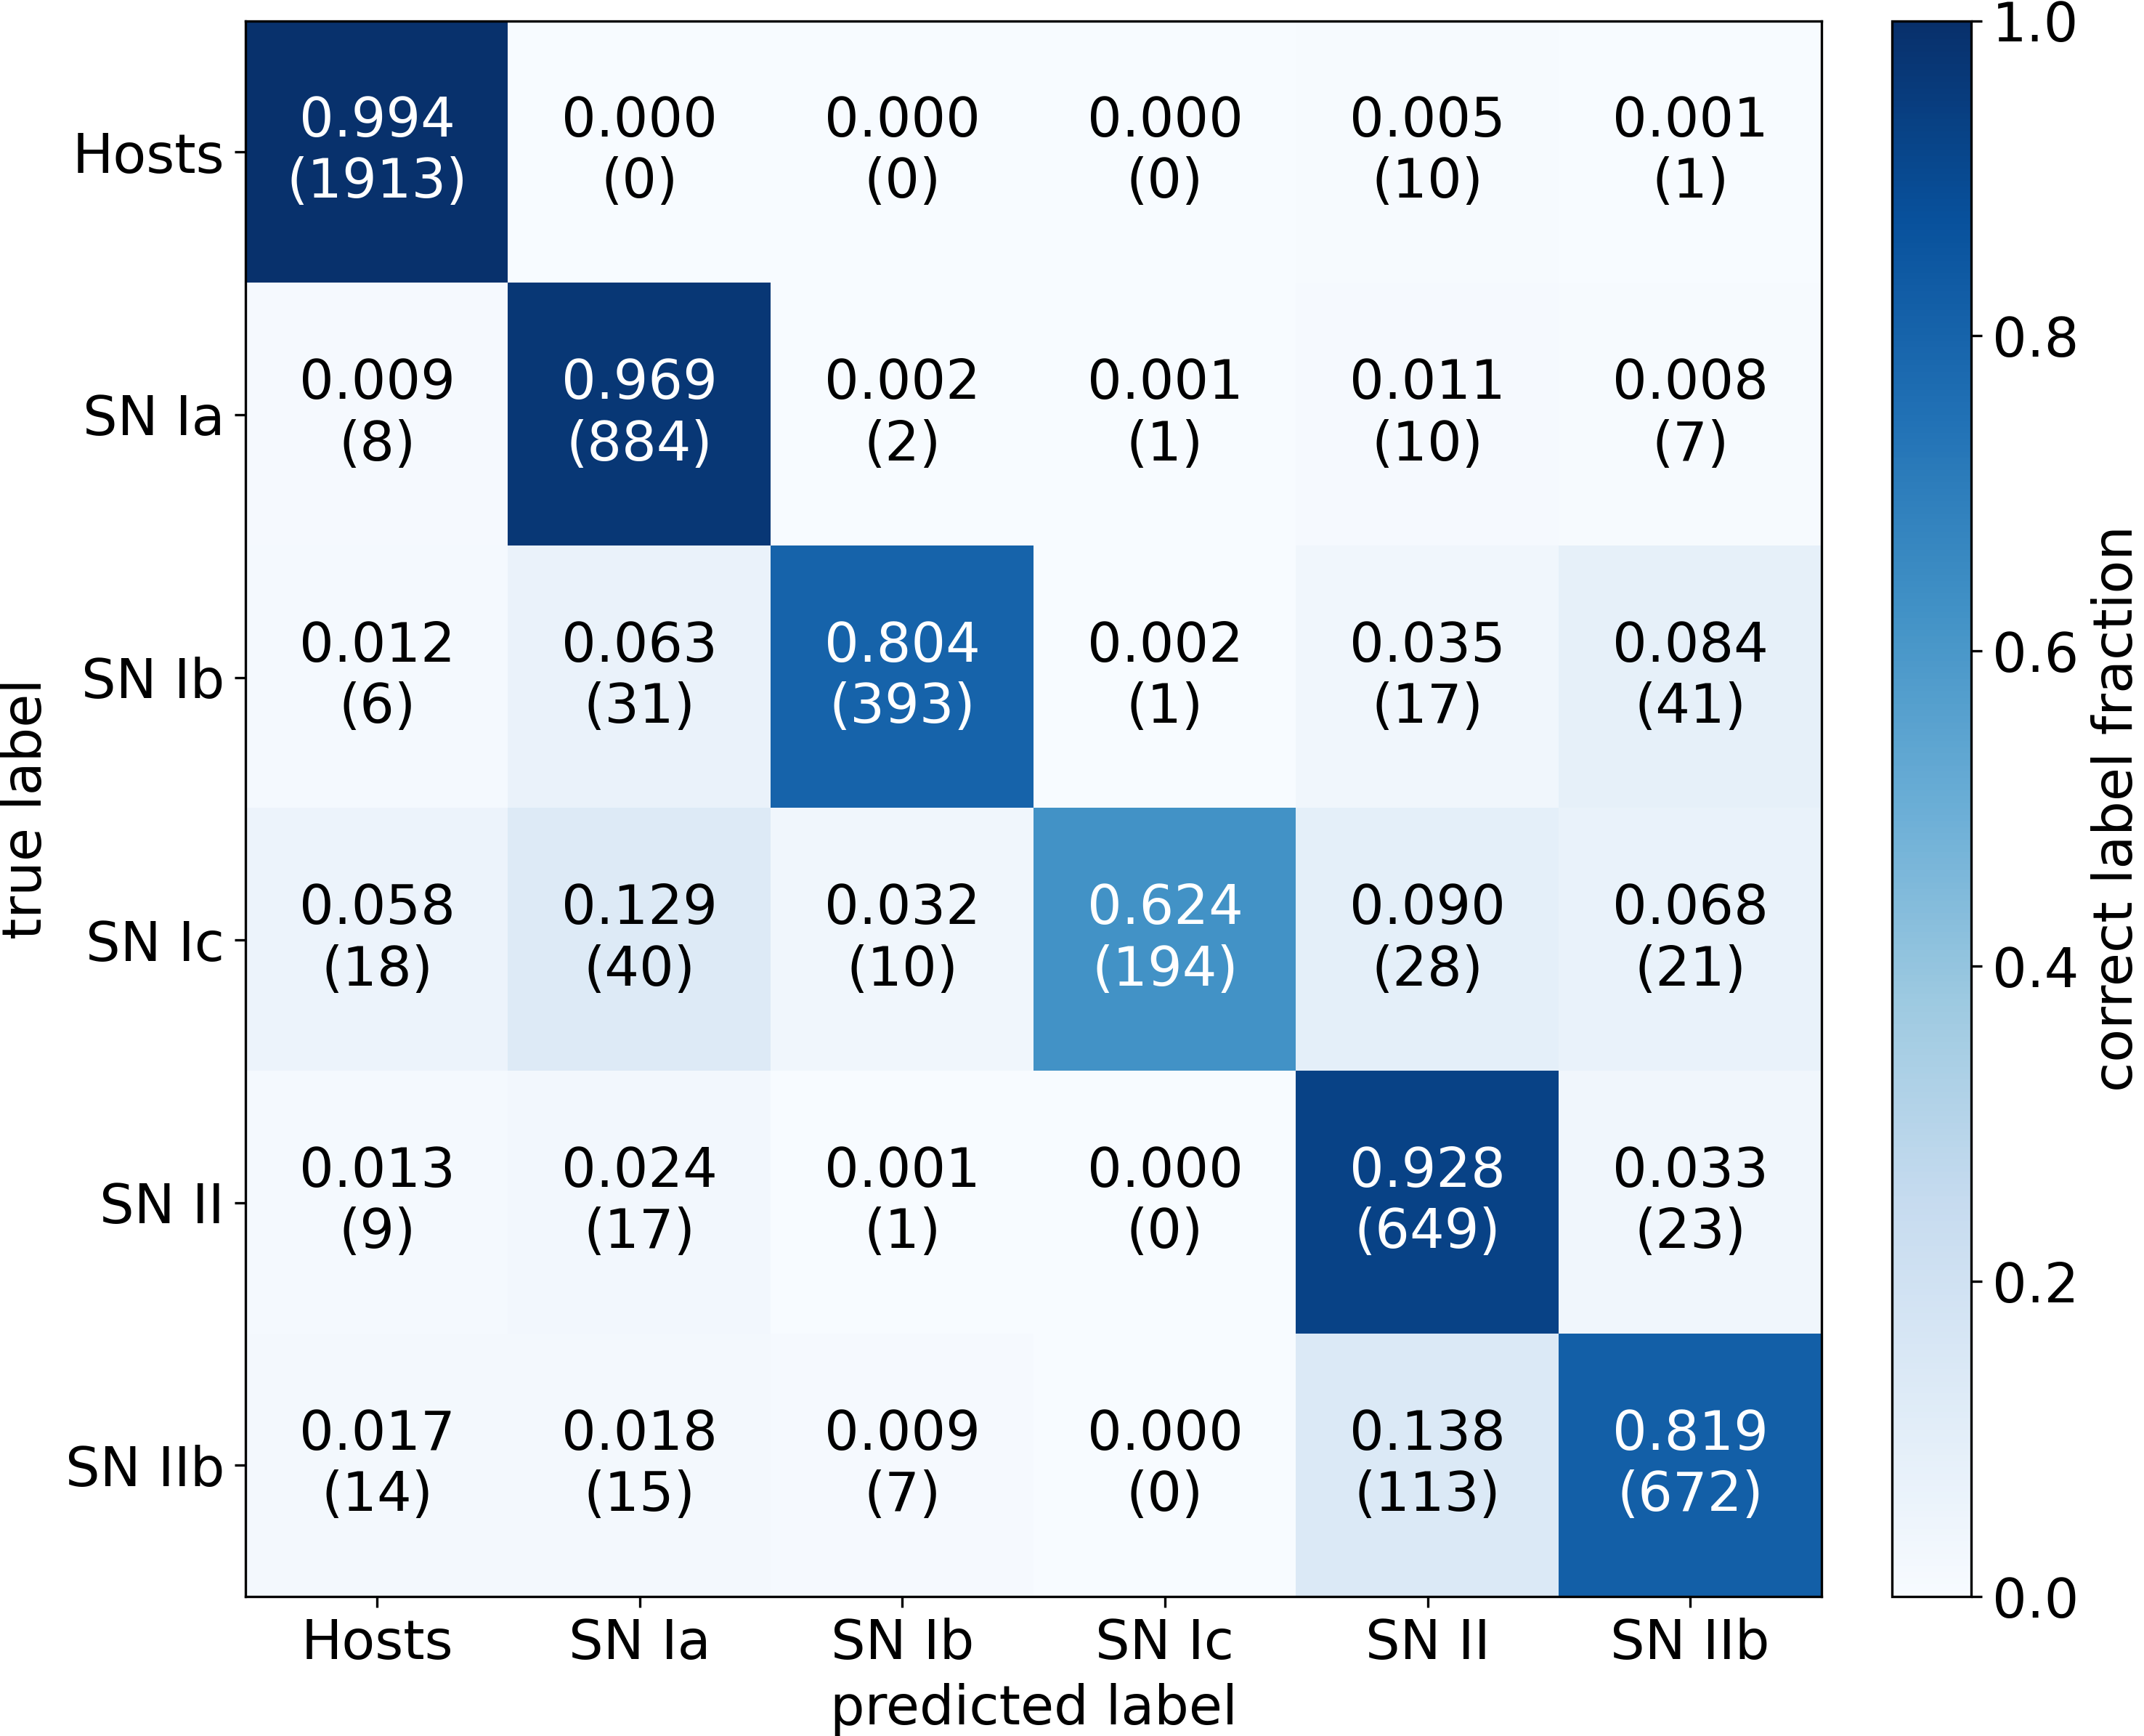
\includegraphics[height=4.3cm]{figures/v1_real/vit_model_V1_original_redocm999999_e31.png}
    \caption{Spectral ViT V1 Diagnostics: ROC Curve (left) and Confusion Matrix (right) with a 99.9999\% confidence
    cut \label{fig:v1_999999_qual}}
\end{figure}




\clearpage
\section{V2}

\begin{figure}
    \centering
    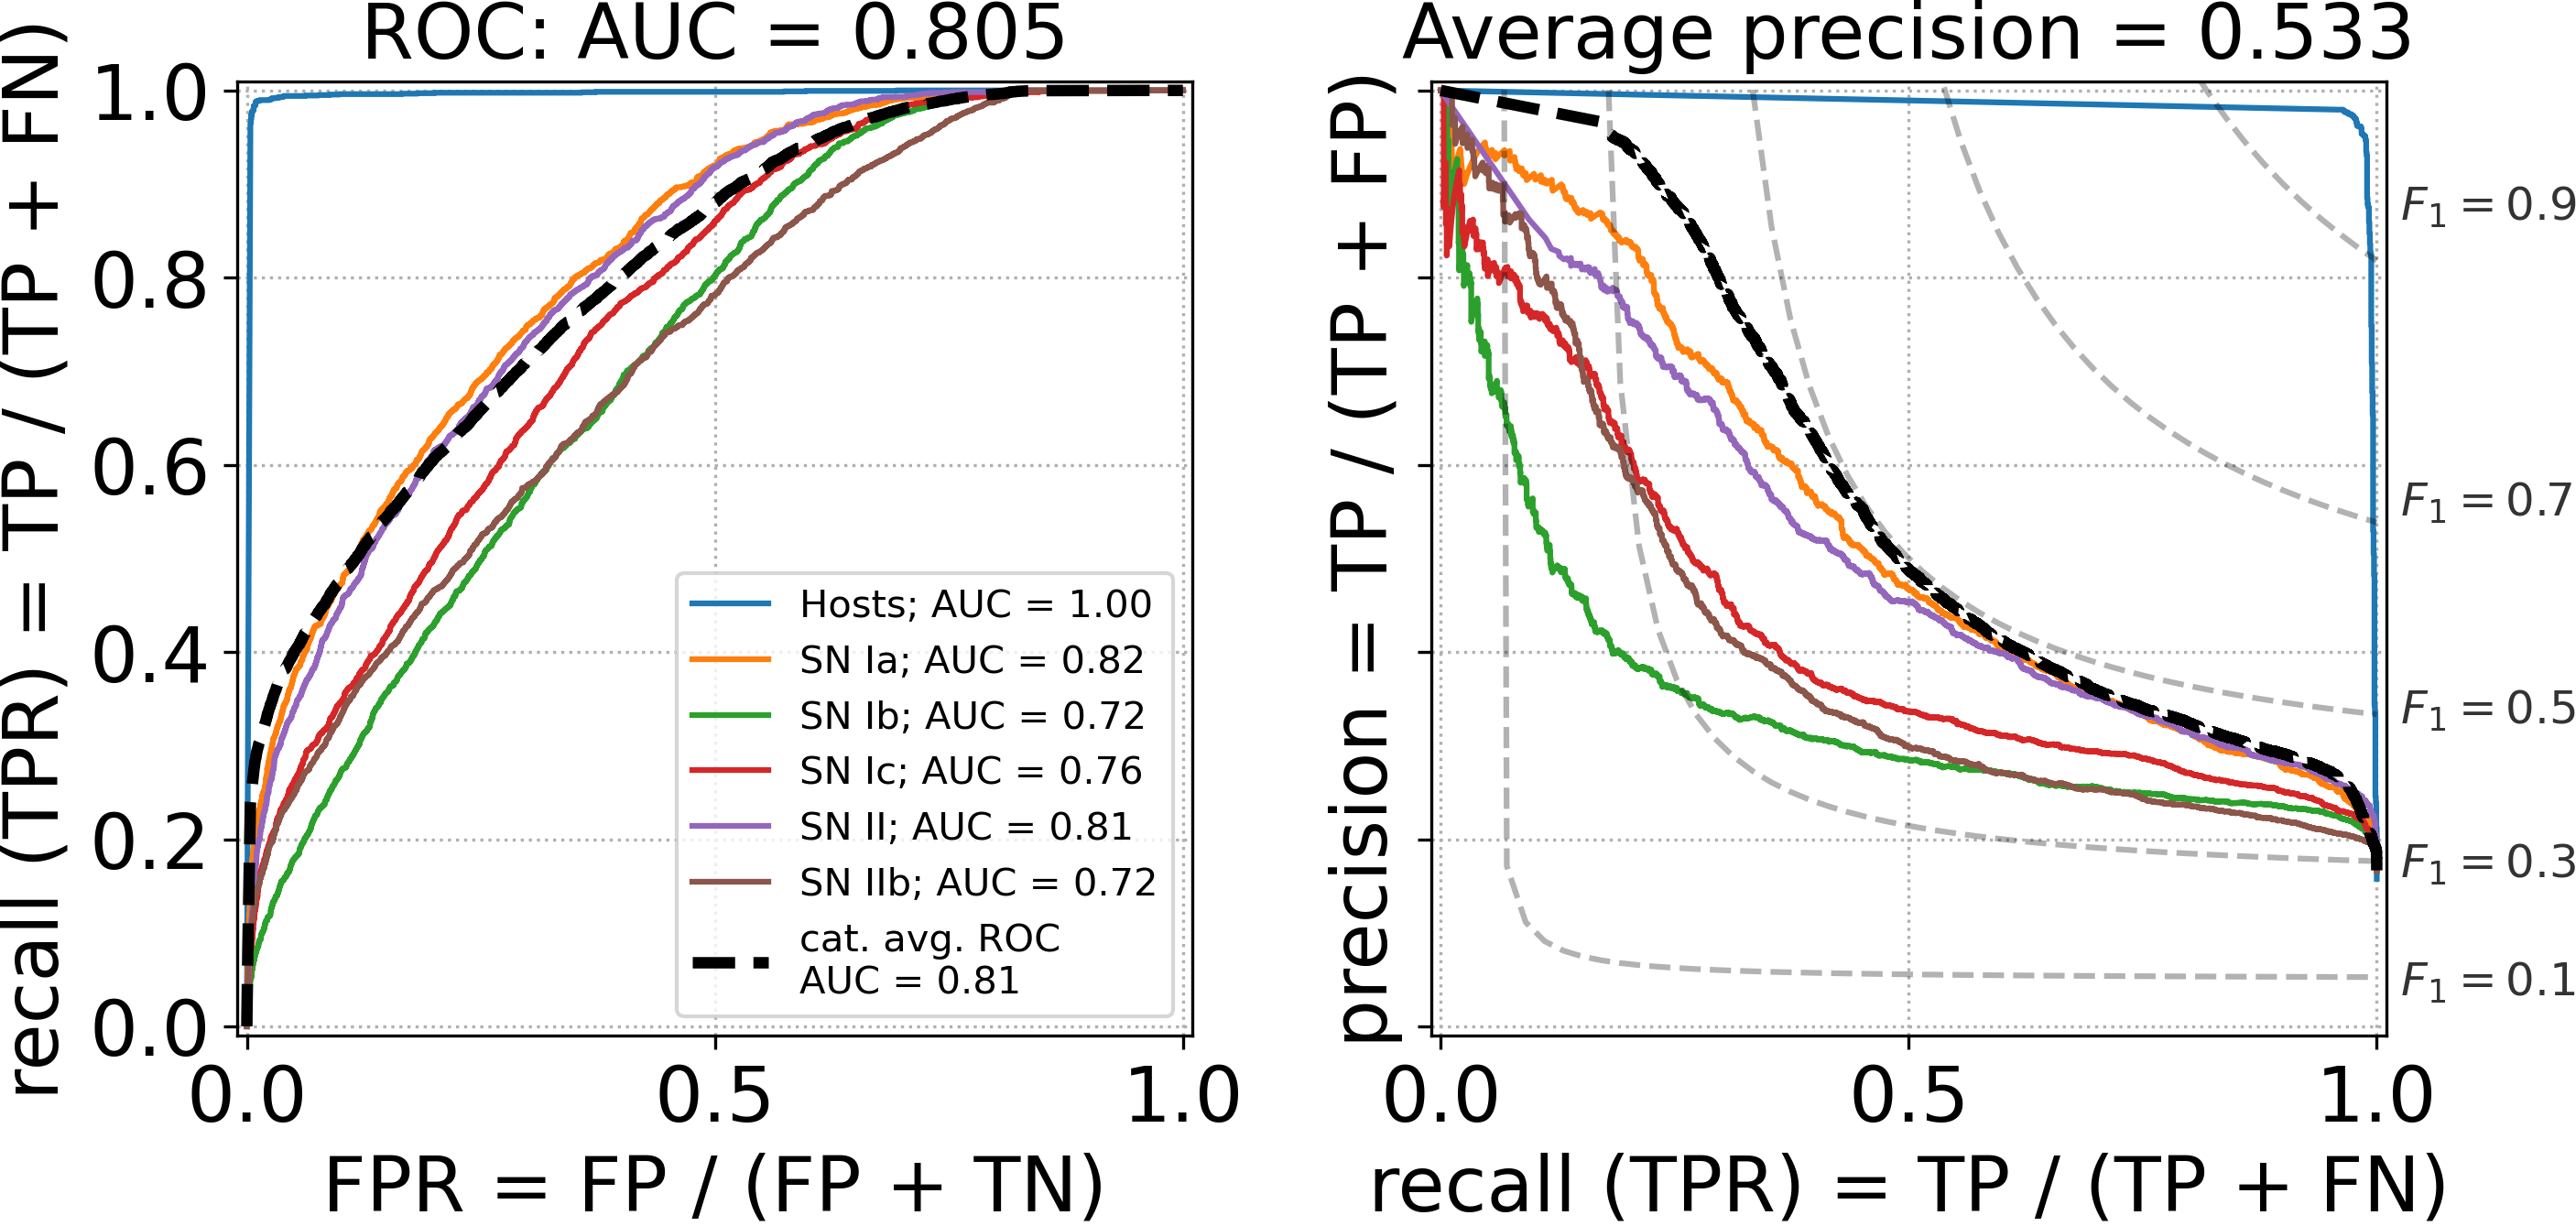
\includegraphics[height=4.3cm]{figures/v2_real/vit_model_V2rocfulle_e26.png}
    \quad
    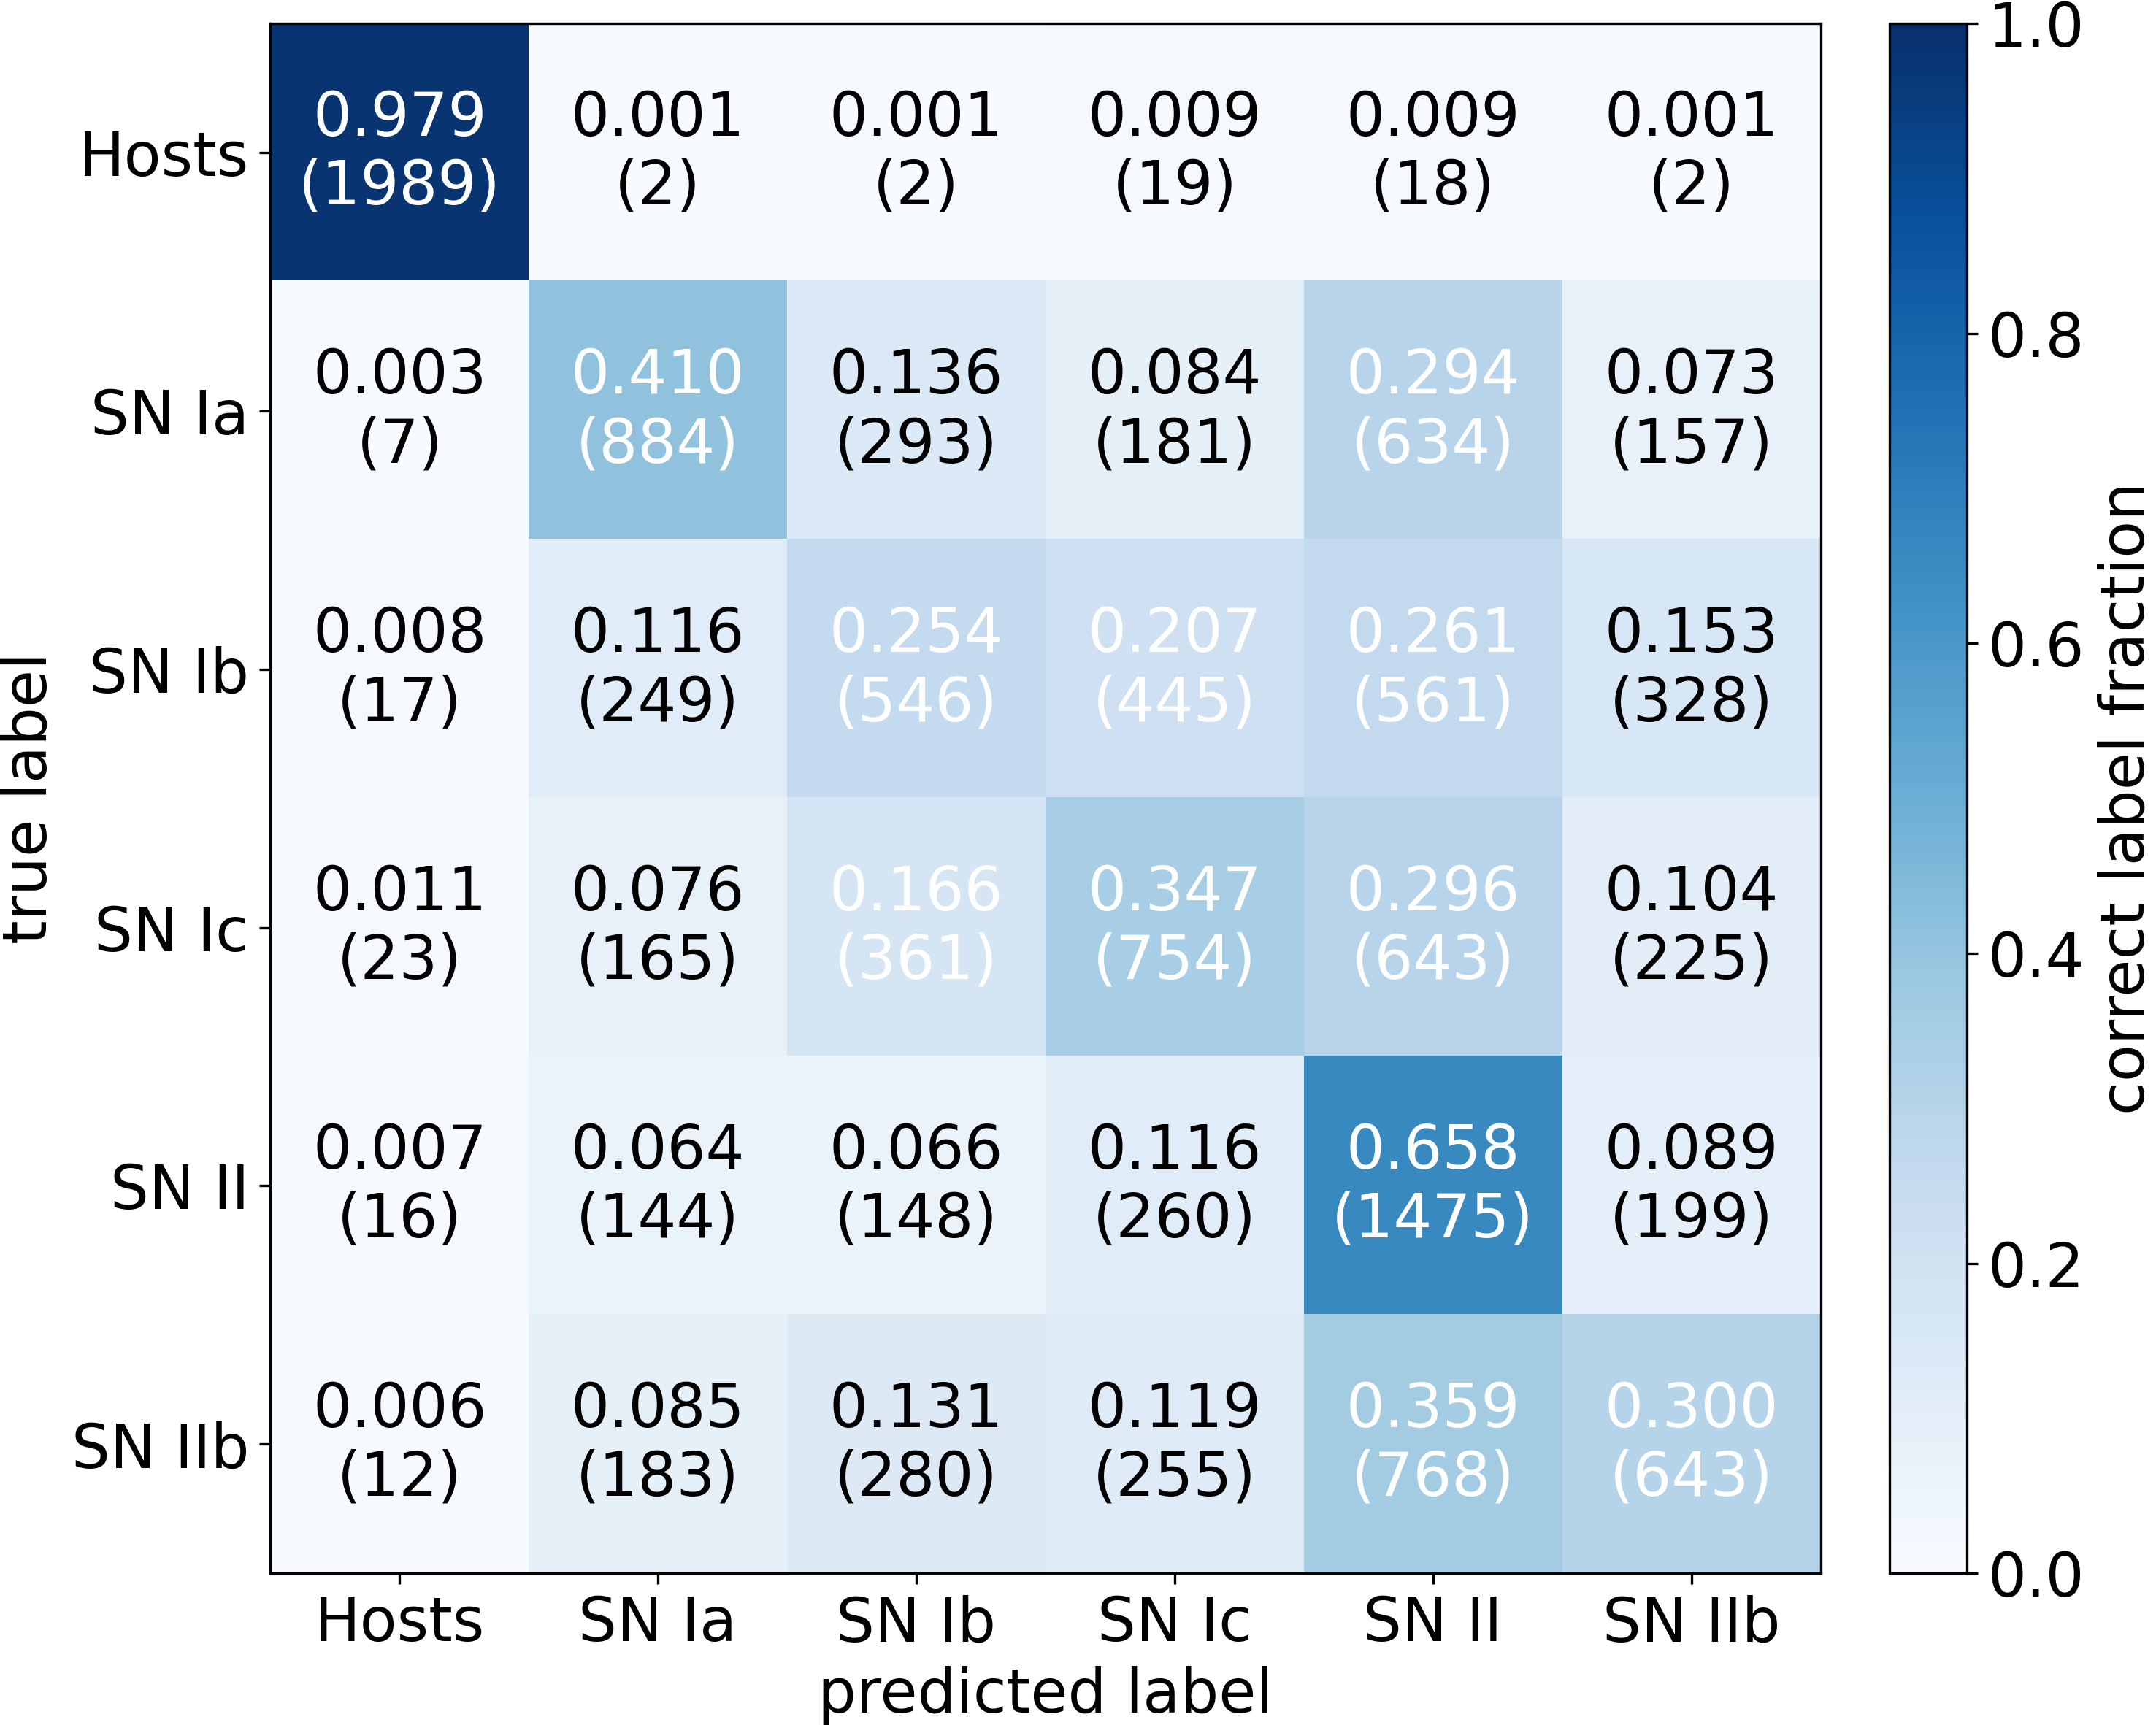
\includegraphics[height=4.3cm]{figures/v2_real/vit_model_V2cmfull_e26.png}
    \caption{Spectral ViT V2 Diagnostics: ROC Curve (left) and Confusion Matrix (right)\label{fig:v2_qual}}
\end{figure}

\begin{figure}
    \centering
    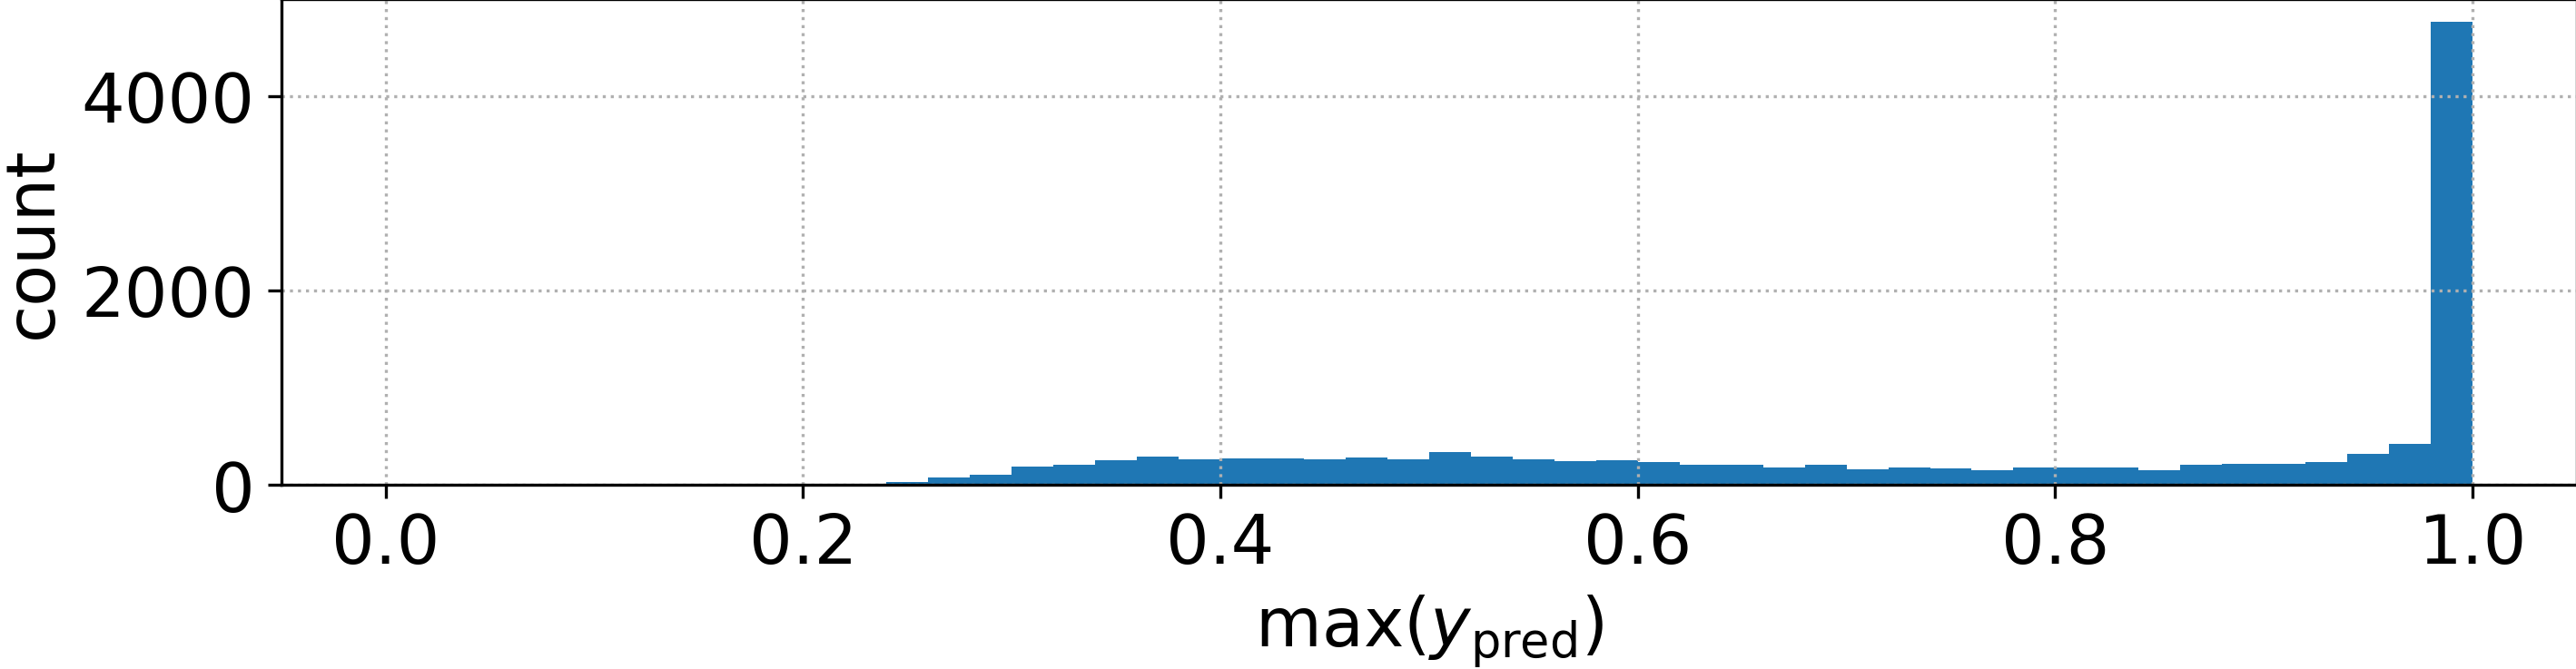
\includegraphics[width=0.6\textwidth]{figures/v2_real/vit_model_V2max_ypred_26.png}
    \caption{Max value of the output vector from the Spectral ViT V2.\label{fig:v2_max}}
\end{figure}

\begin{figure}
    \centering
    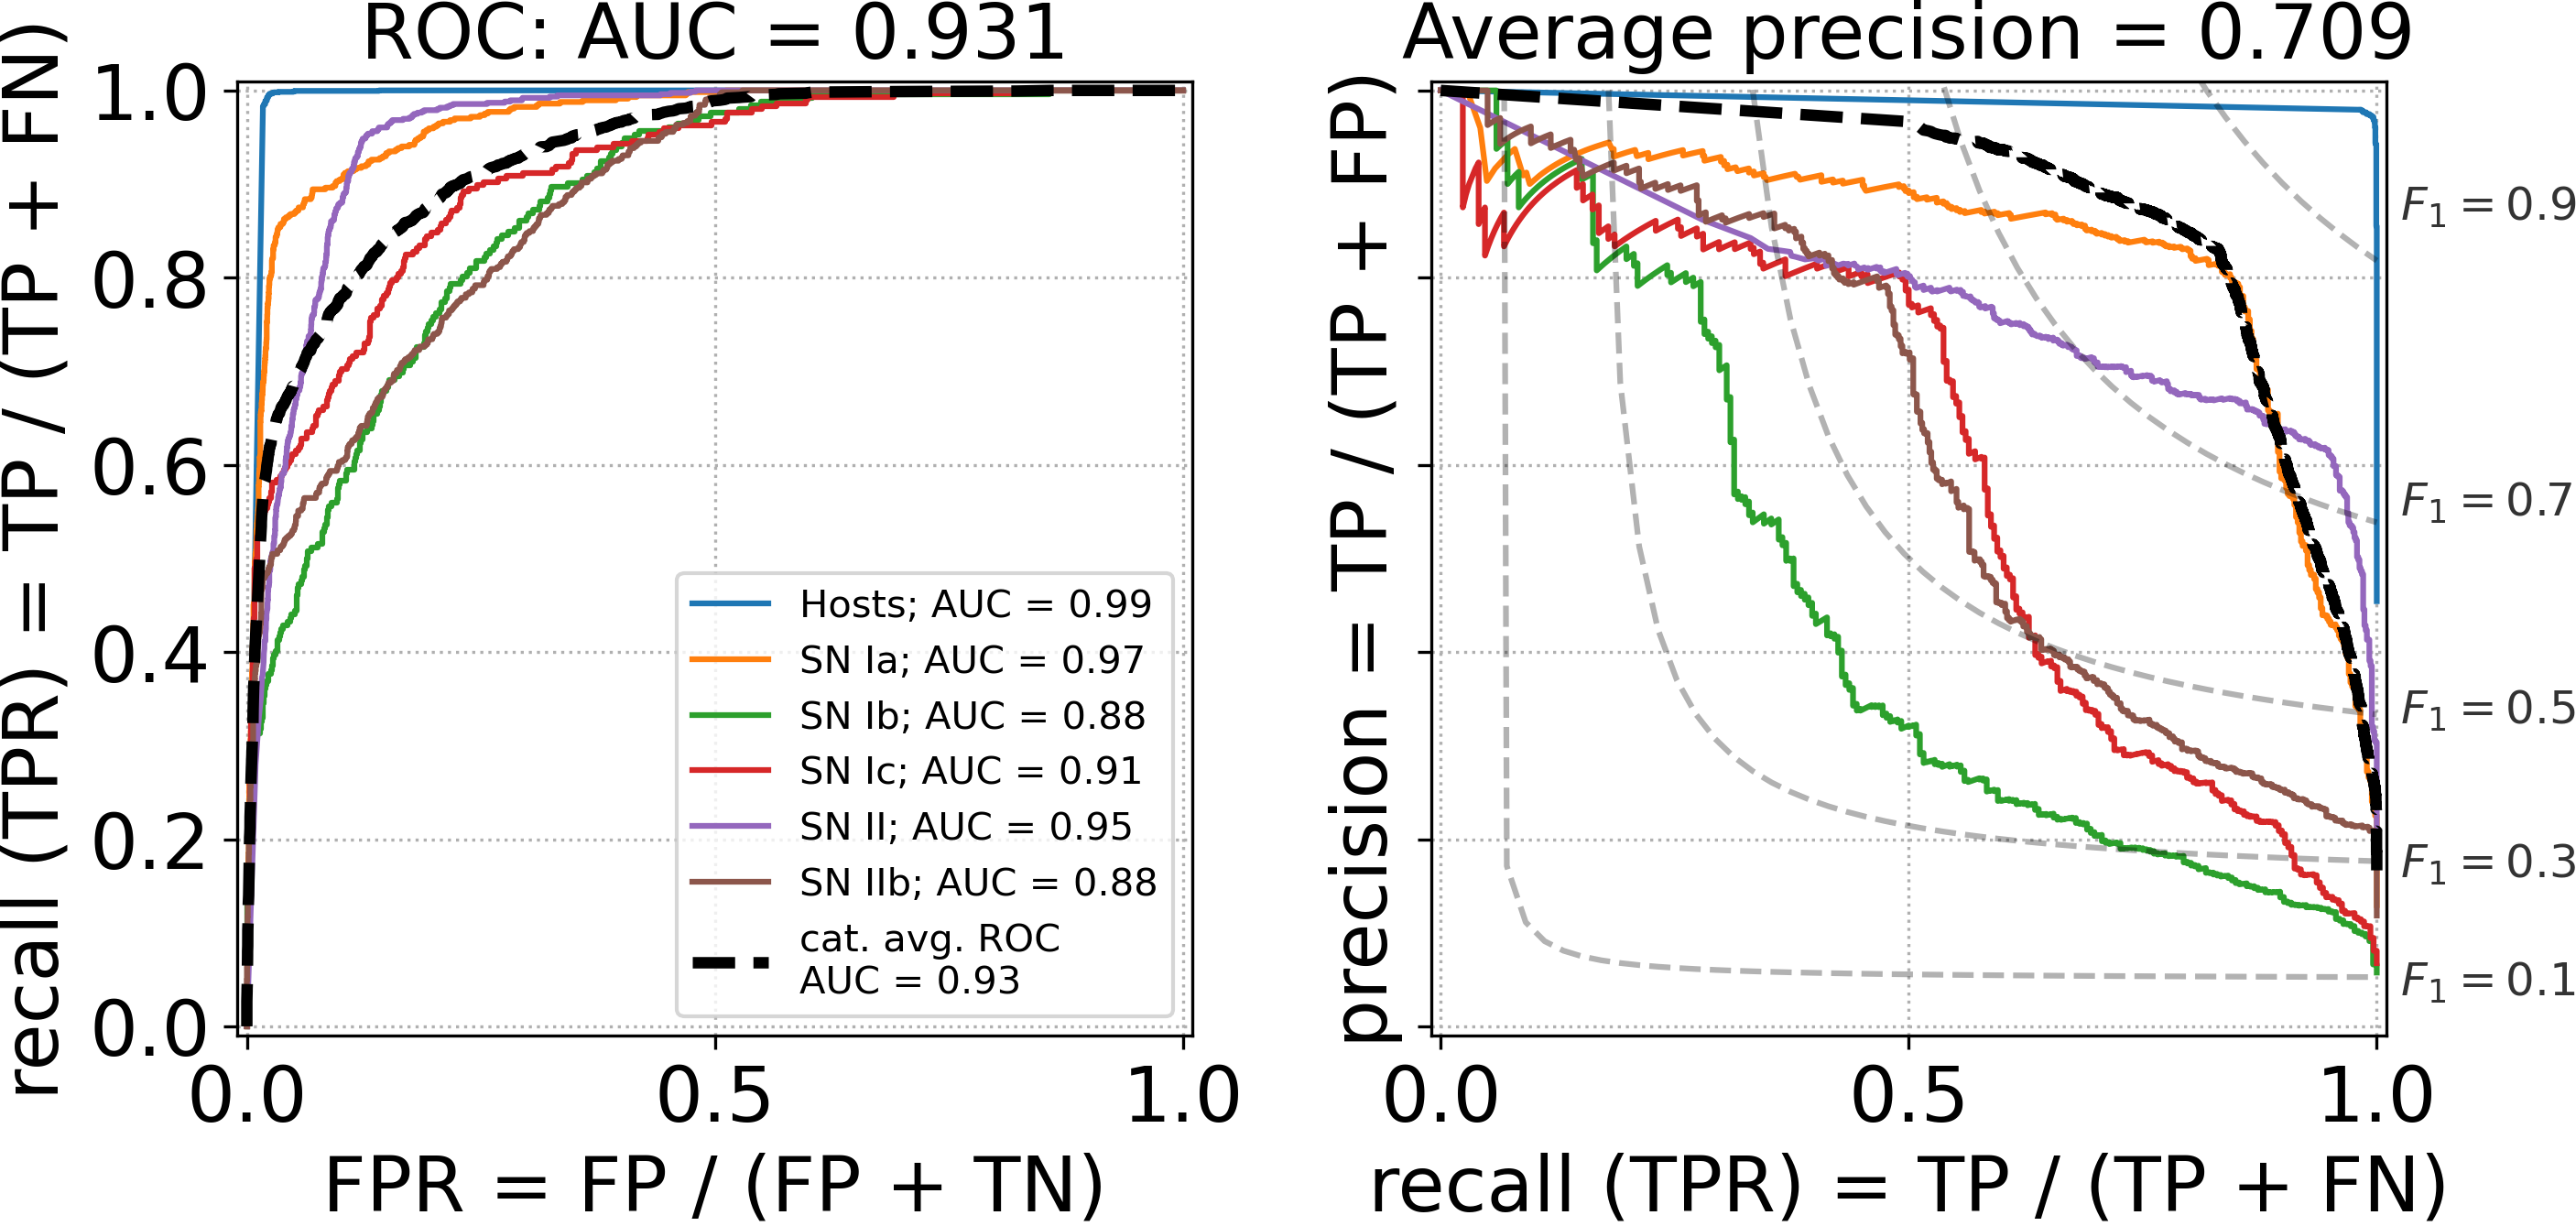
\includegraphics[height=4.3cm]{figures/v2_real/vit_model_V2roc99_e26.png}
    \quad
    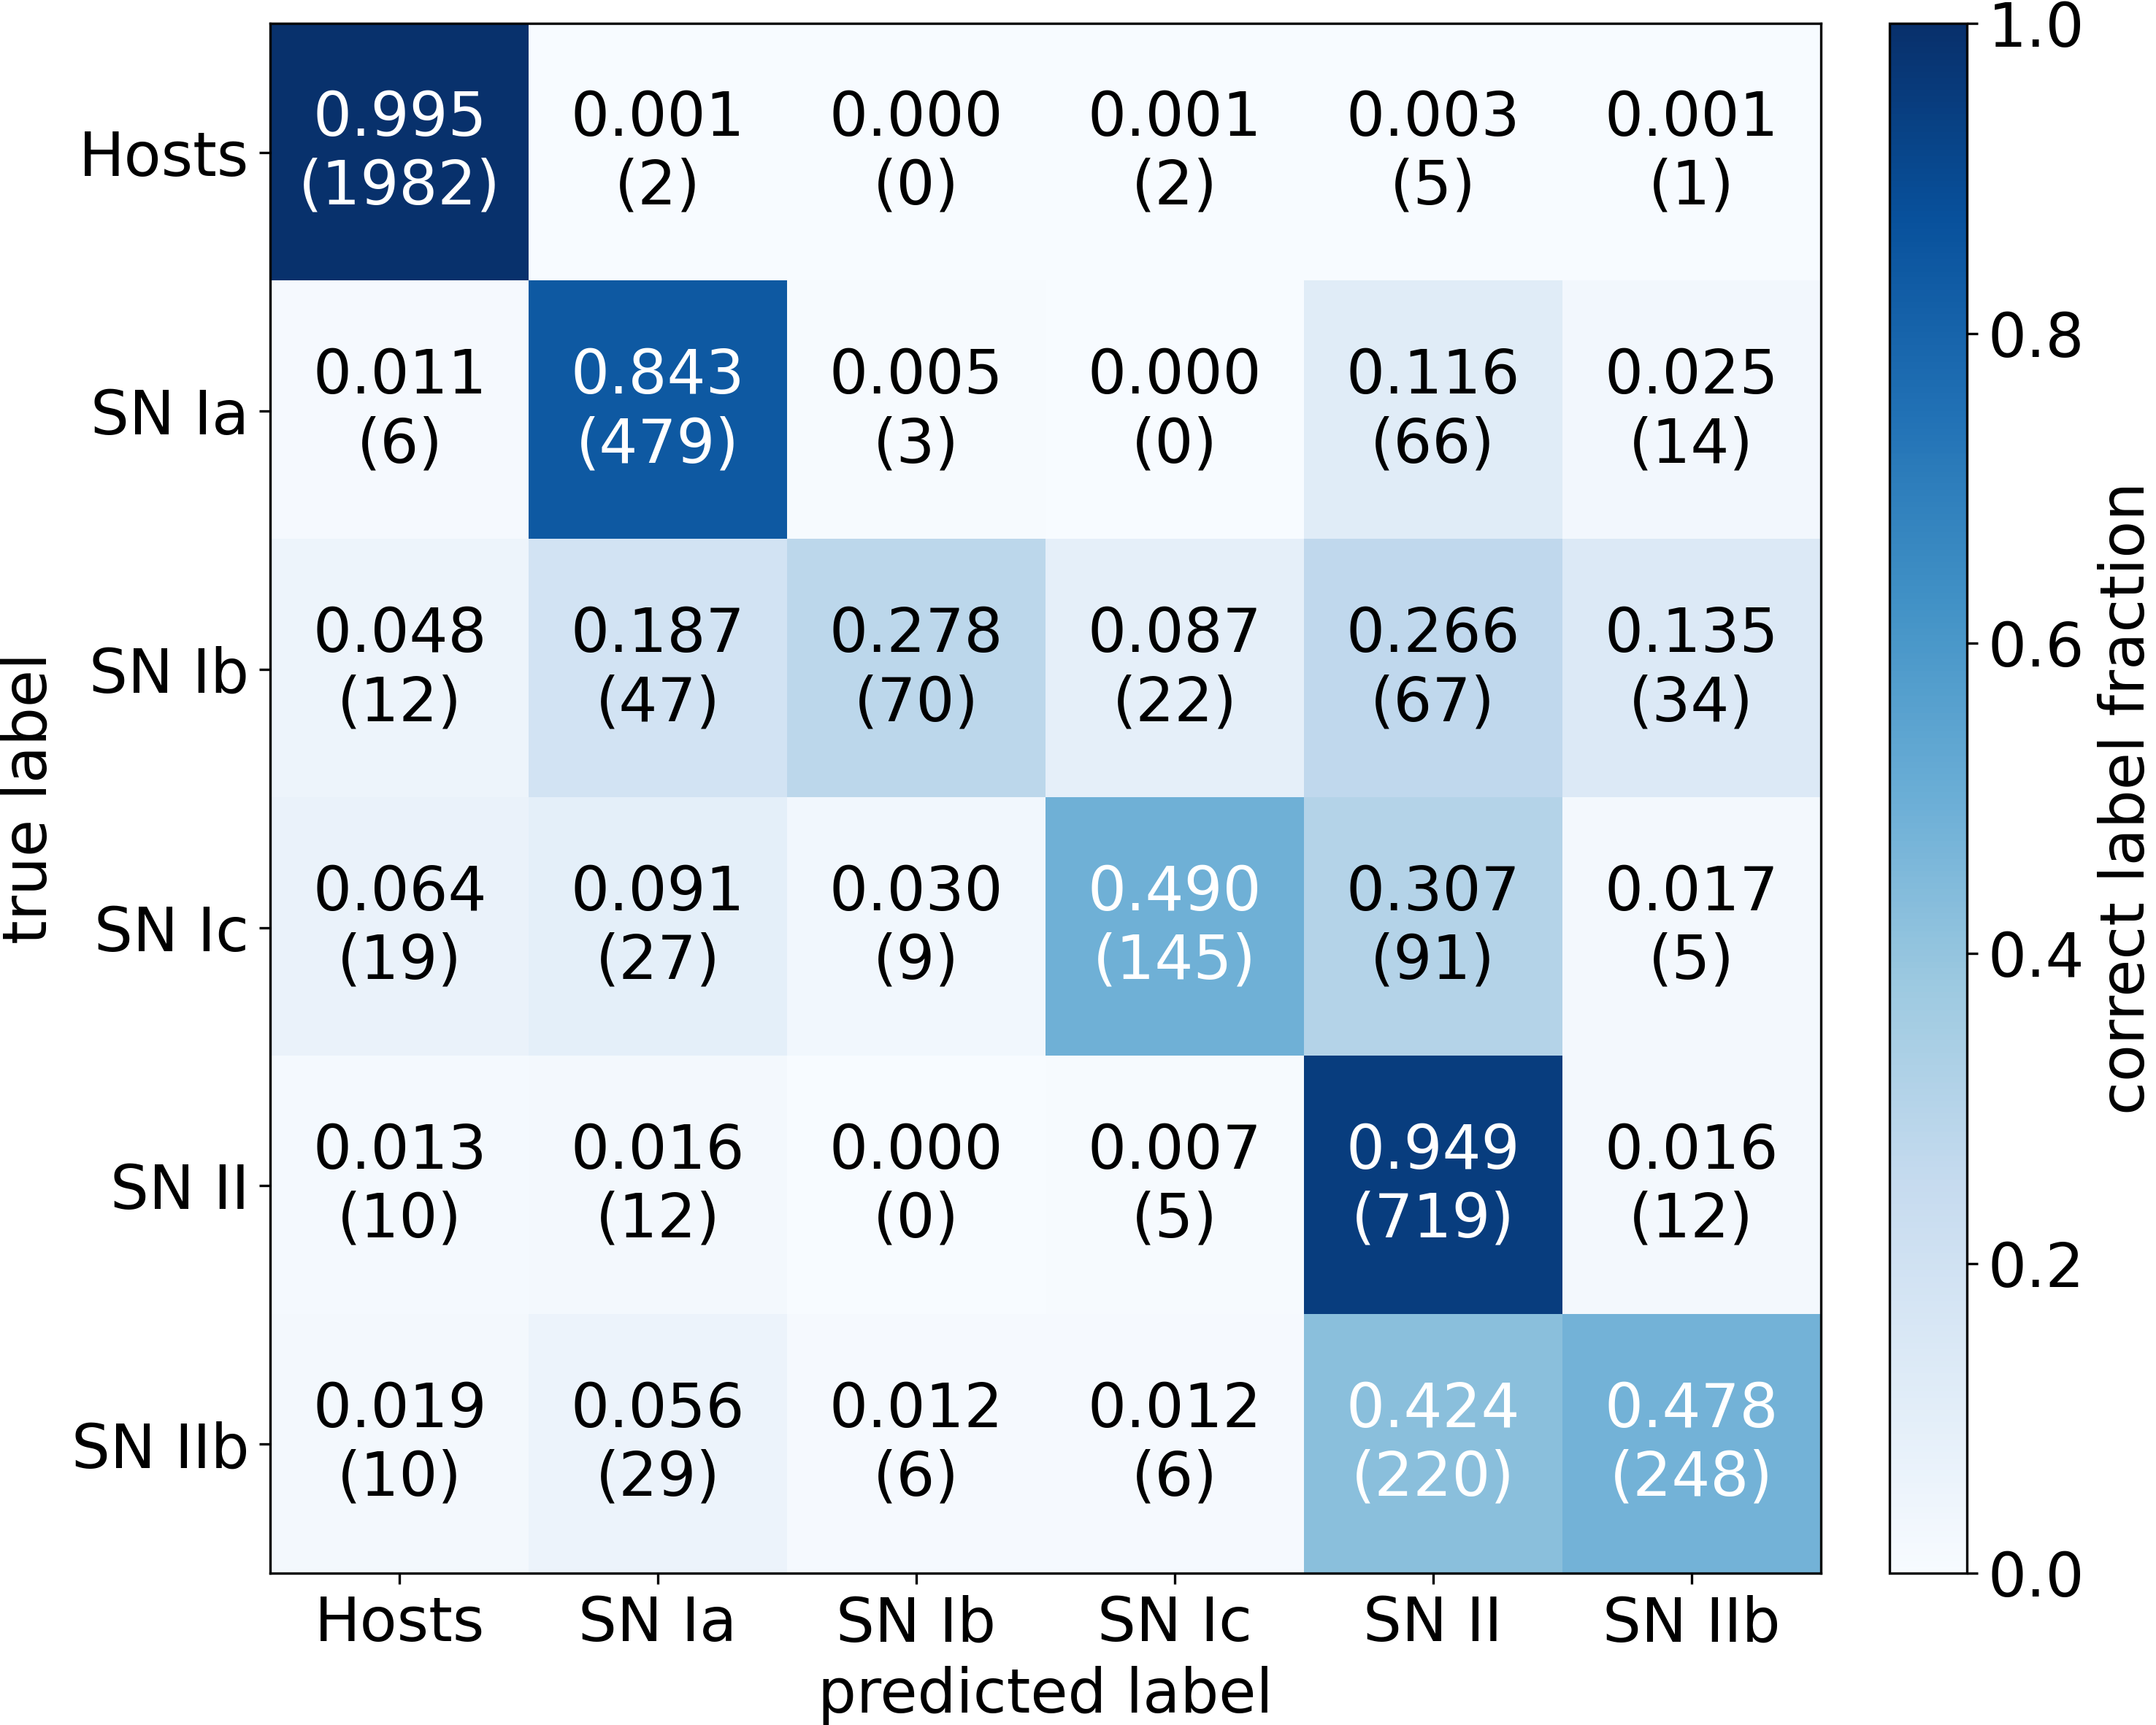
\includegraphics[height=4.3cm]{figures/v2_real/vit_model_V2cm99_e26.png}
    \caption{Spectral ViT V2 Diagnostics: ROC Curve (left) and Confusion Matrix (right) with a 99\% confidence
    cut\label{fig:v2_99_qual}}
\end{figure}



\clearpage
\subsection{Binary Classification}

\begin{figure}
    \centering
    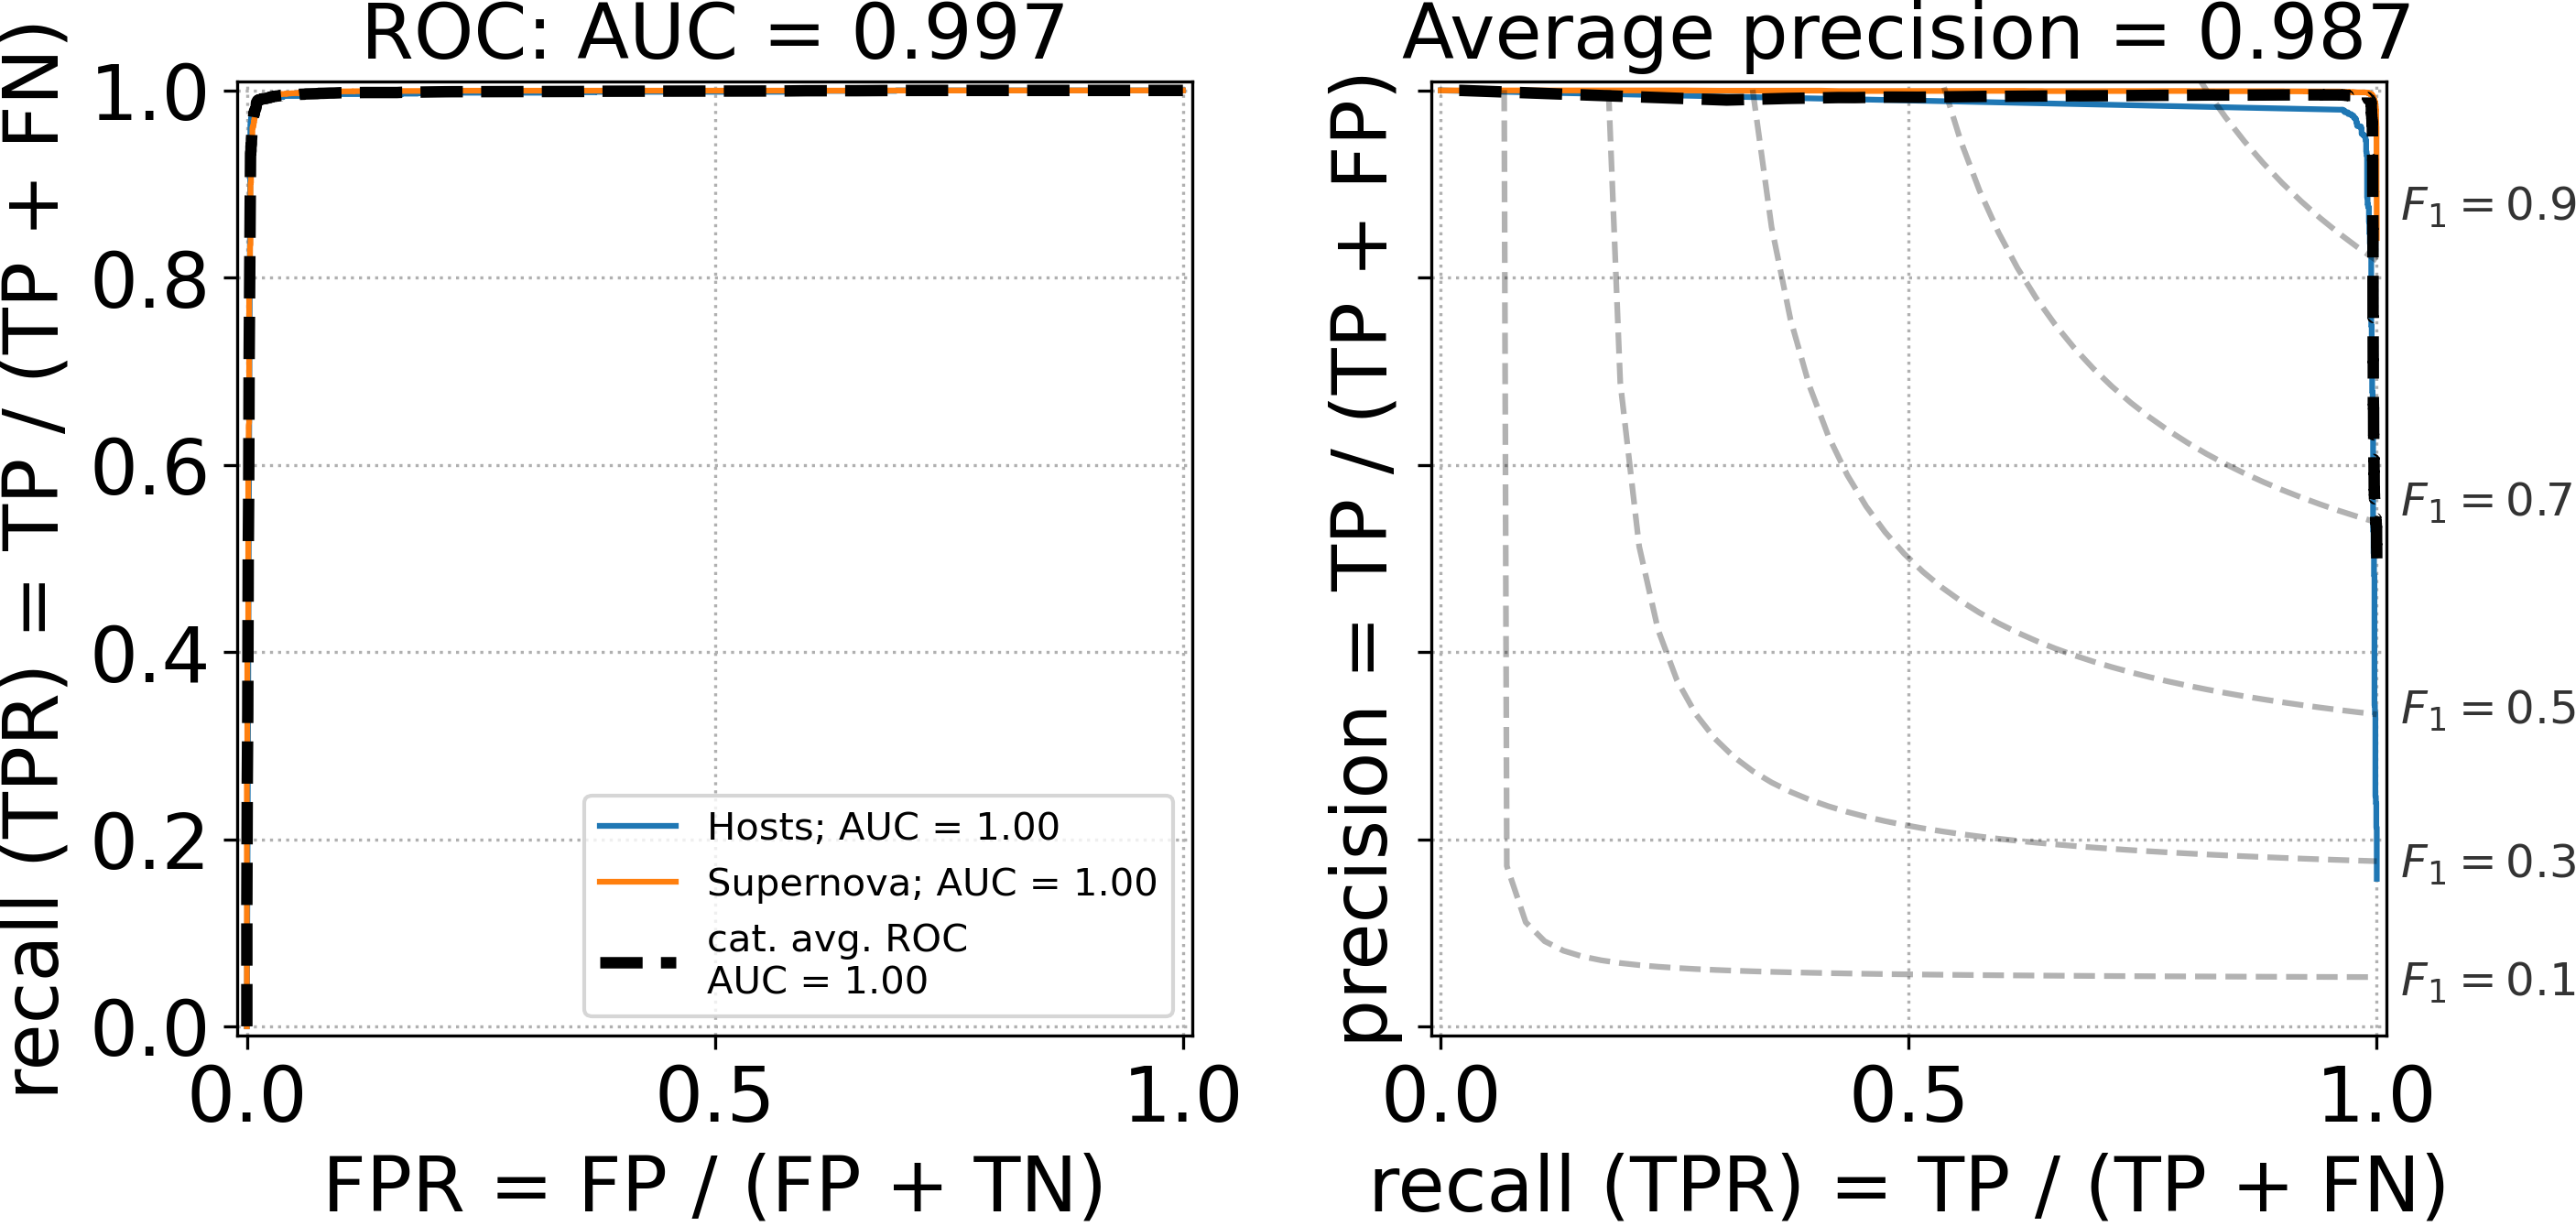
\includegraphics[height=4.2cm]{figures/v2_real/vit_model_V2rocfull_binary_e26.png}
    \quad
    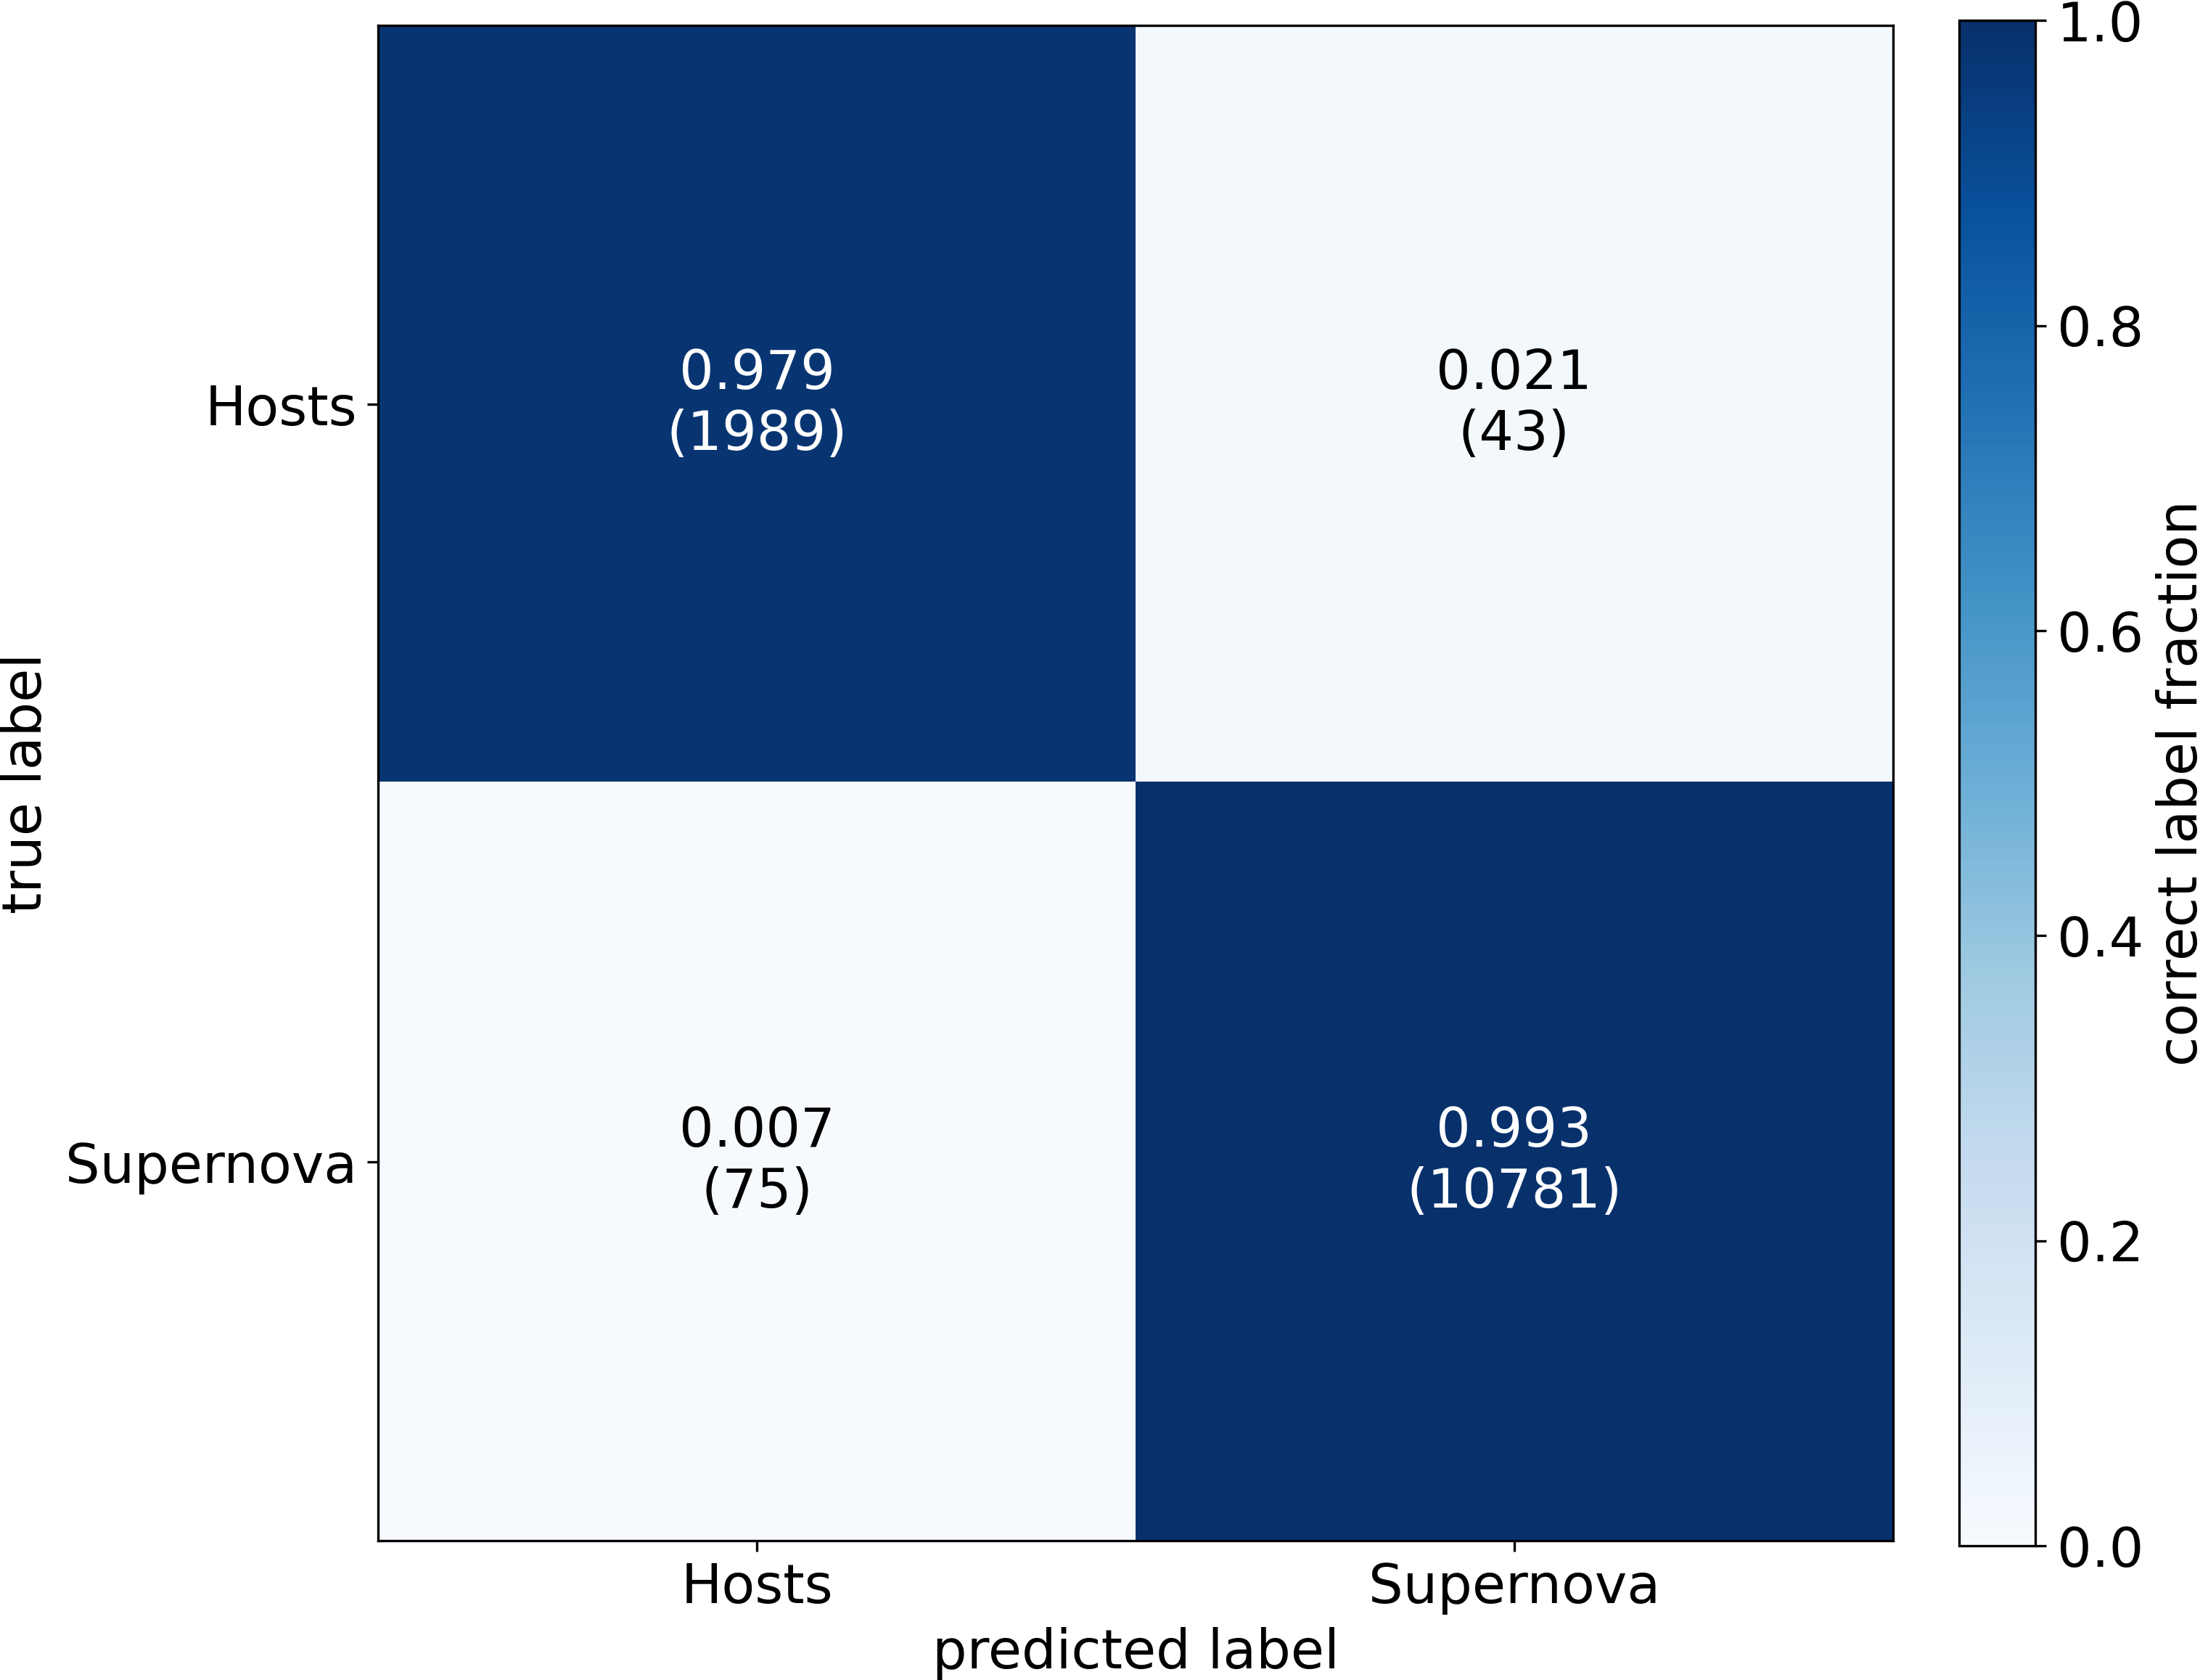
\includegraphics[height=4.2cm]{figures/v2_real/vit_model_V2cmfull_binary_e26.png}
    \caption{Spectral ViT V2 Binary Diagnostics: ROC Curve (left) and Confusion Matrix (right)\label{fig:cnn_qual}}
\end{figure}

\begin{figure}
    \centering
    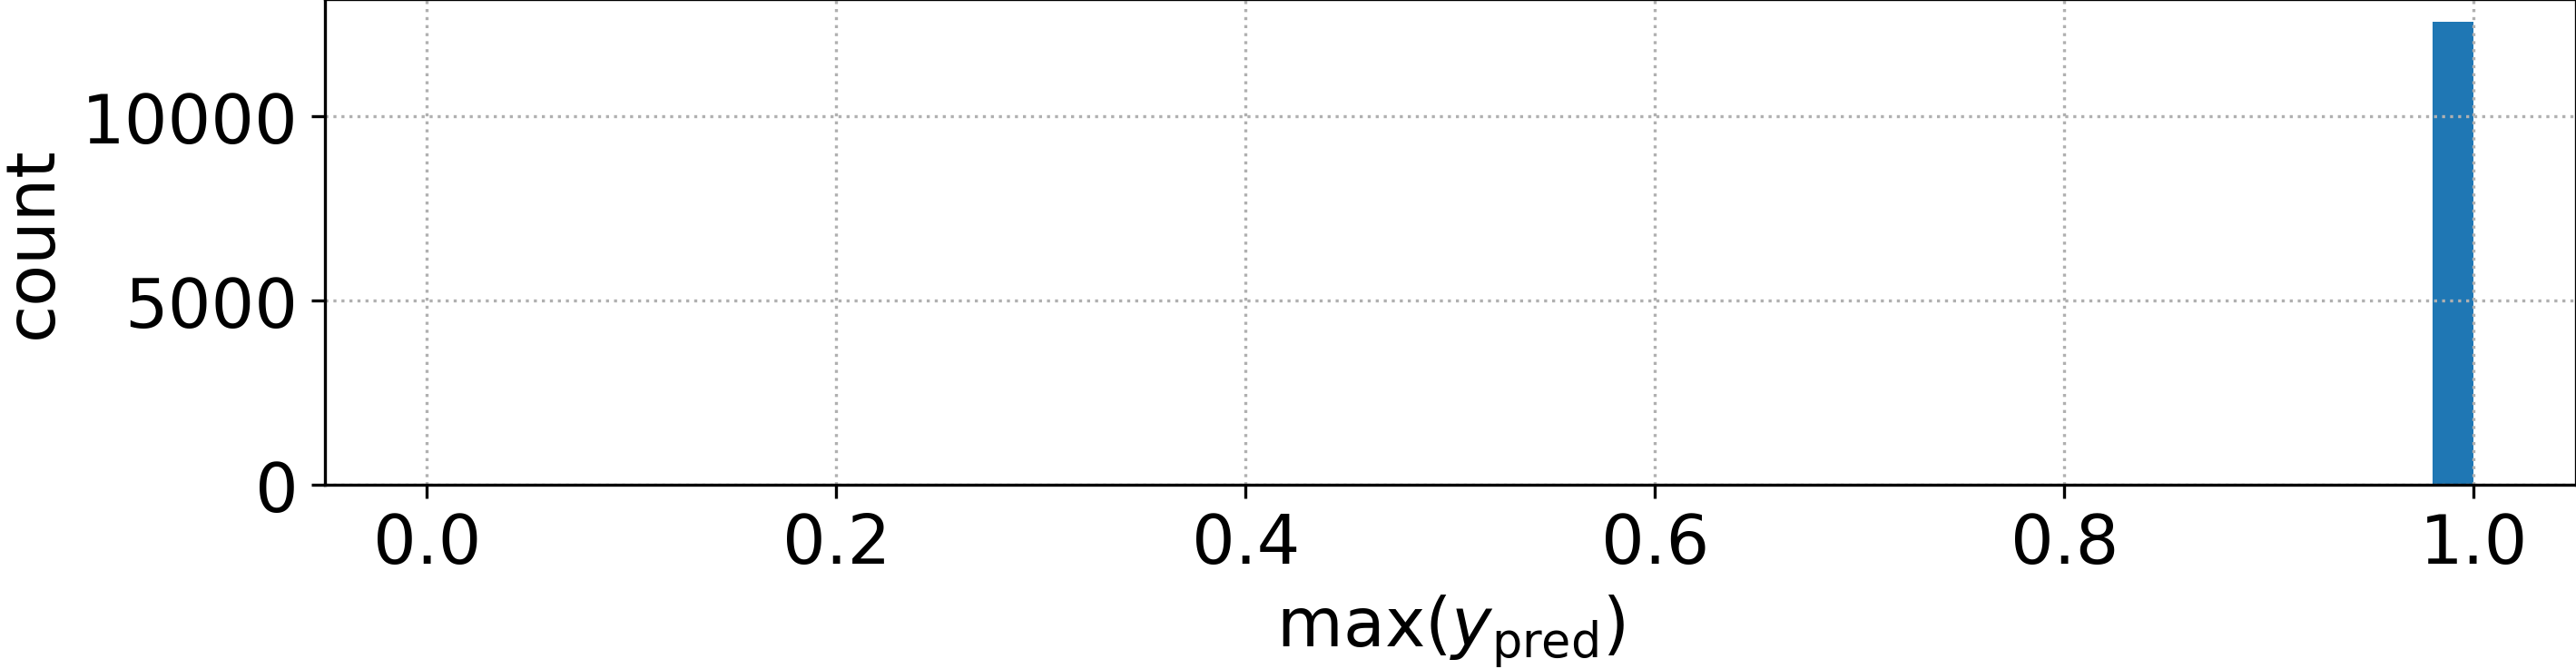
\includegraphics[width=0.6\textwidth]{figures/v2_real/vit_model_V2max_ypred_binary_26.png}
    \caption{Max value of the output vector from the Spectral ViT V2 Binary Classification.\label{fig:cnn_max}}
\end{figure}



\begin{figure}
    \centering
    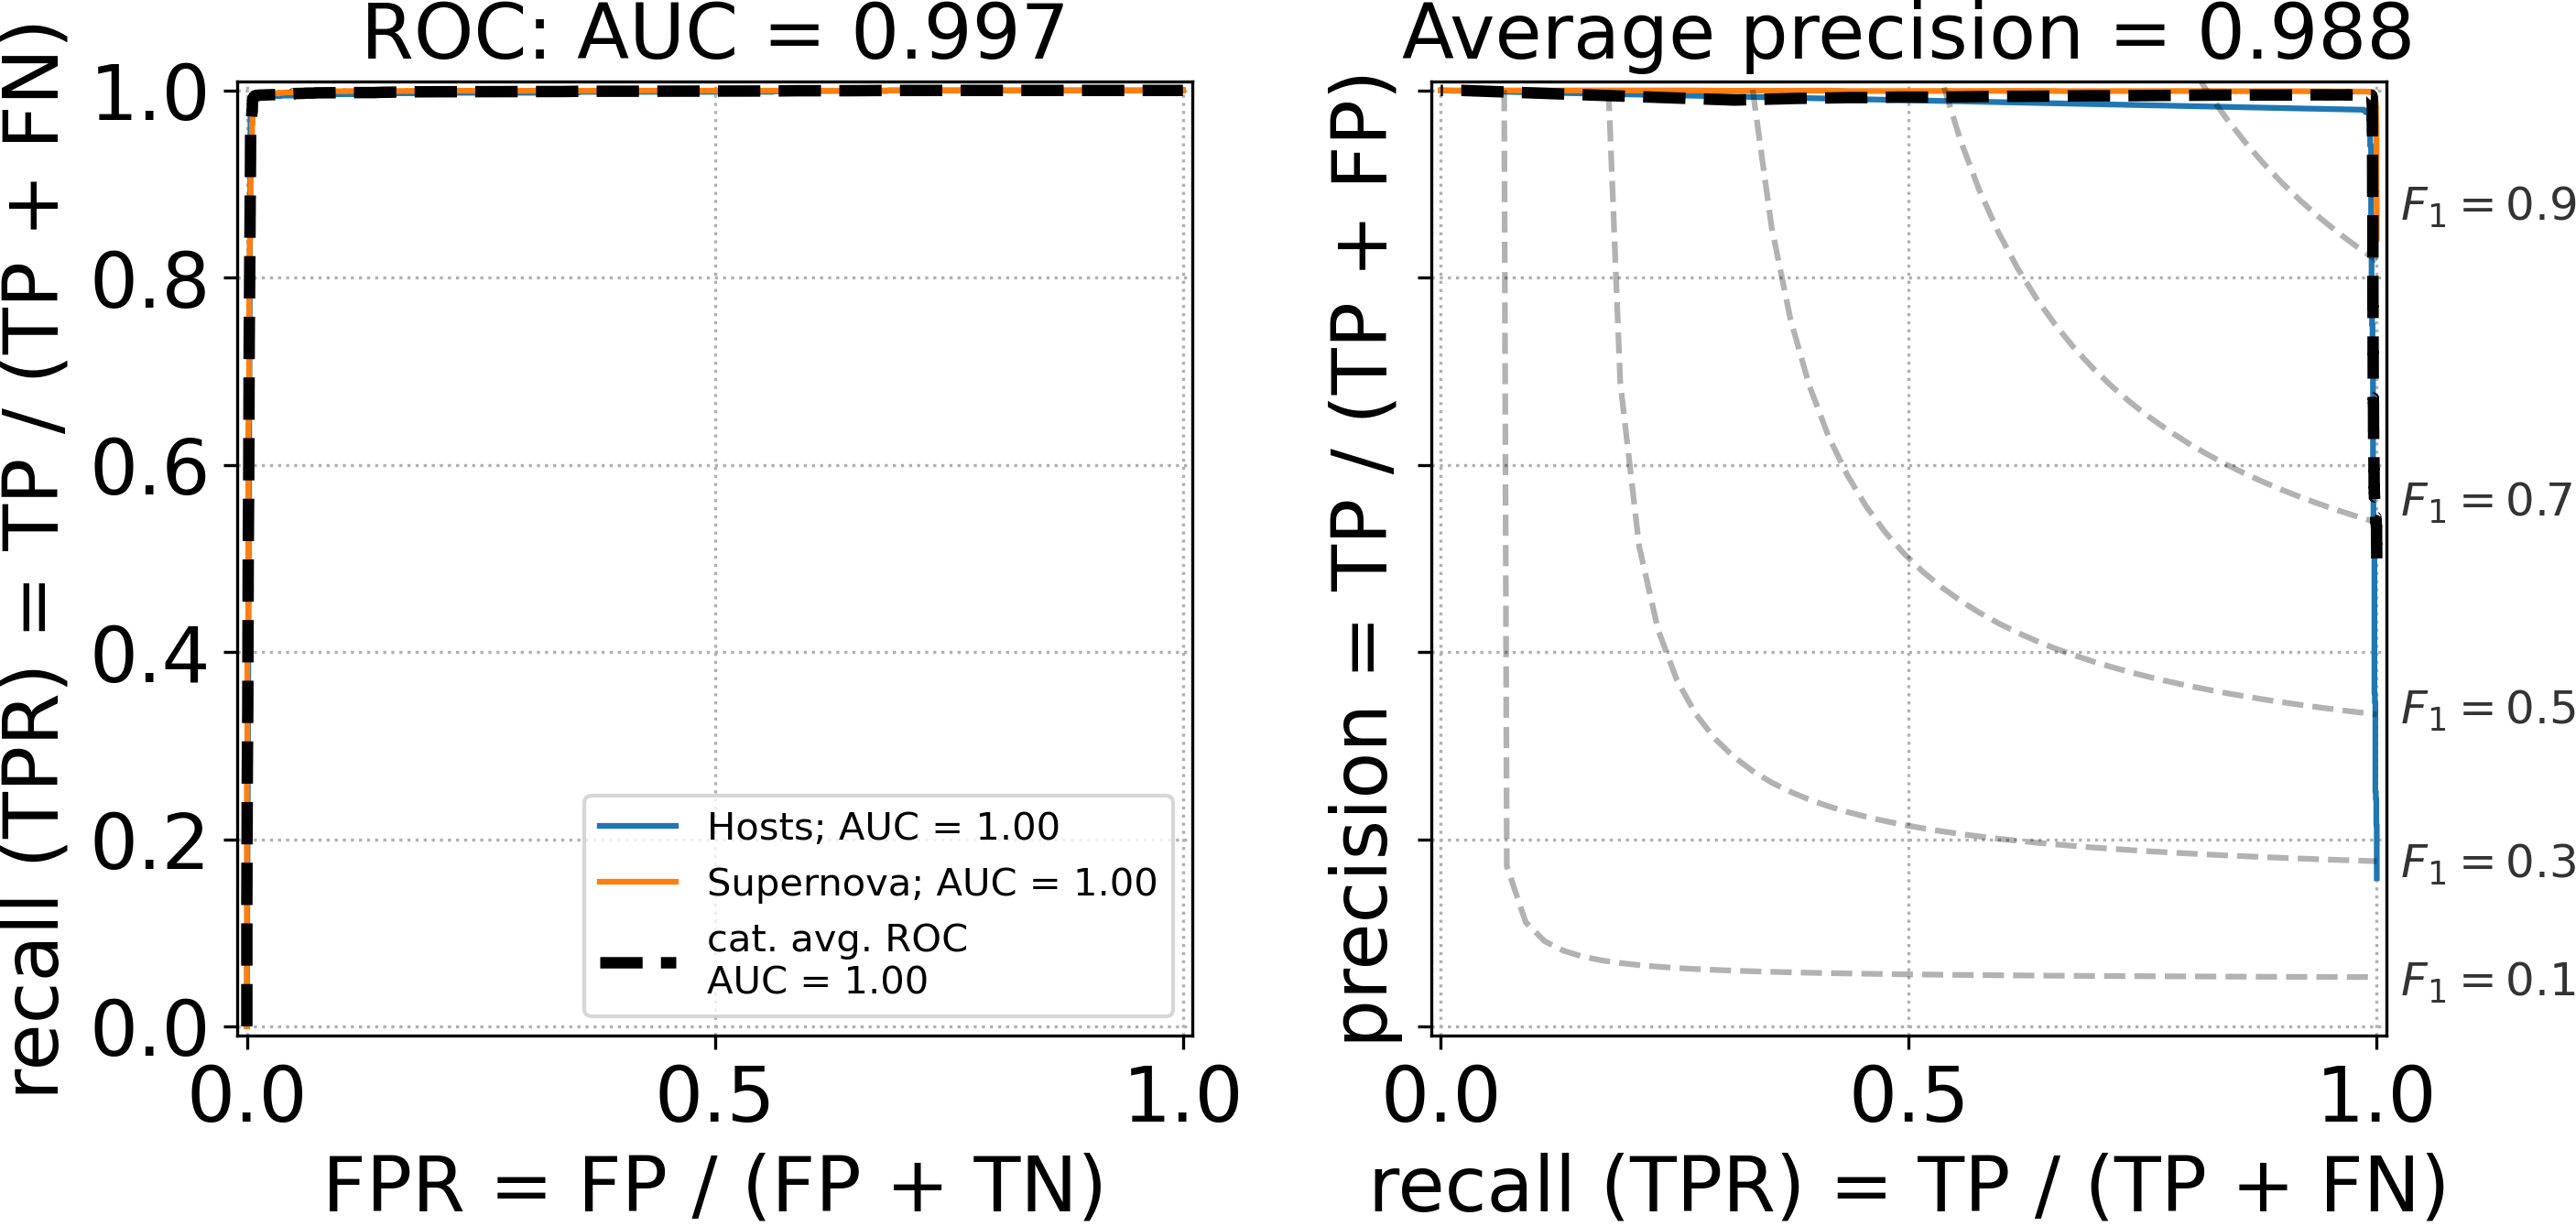
\includegraphics[height=4.2cm]{figures/v2_real/vit_model_V2roc9999_binary_e26.png}
    \quad
    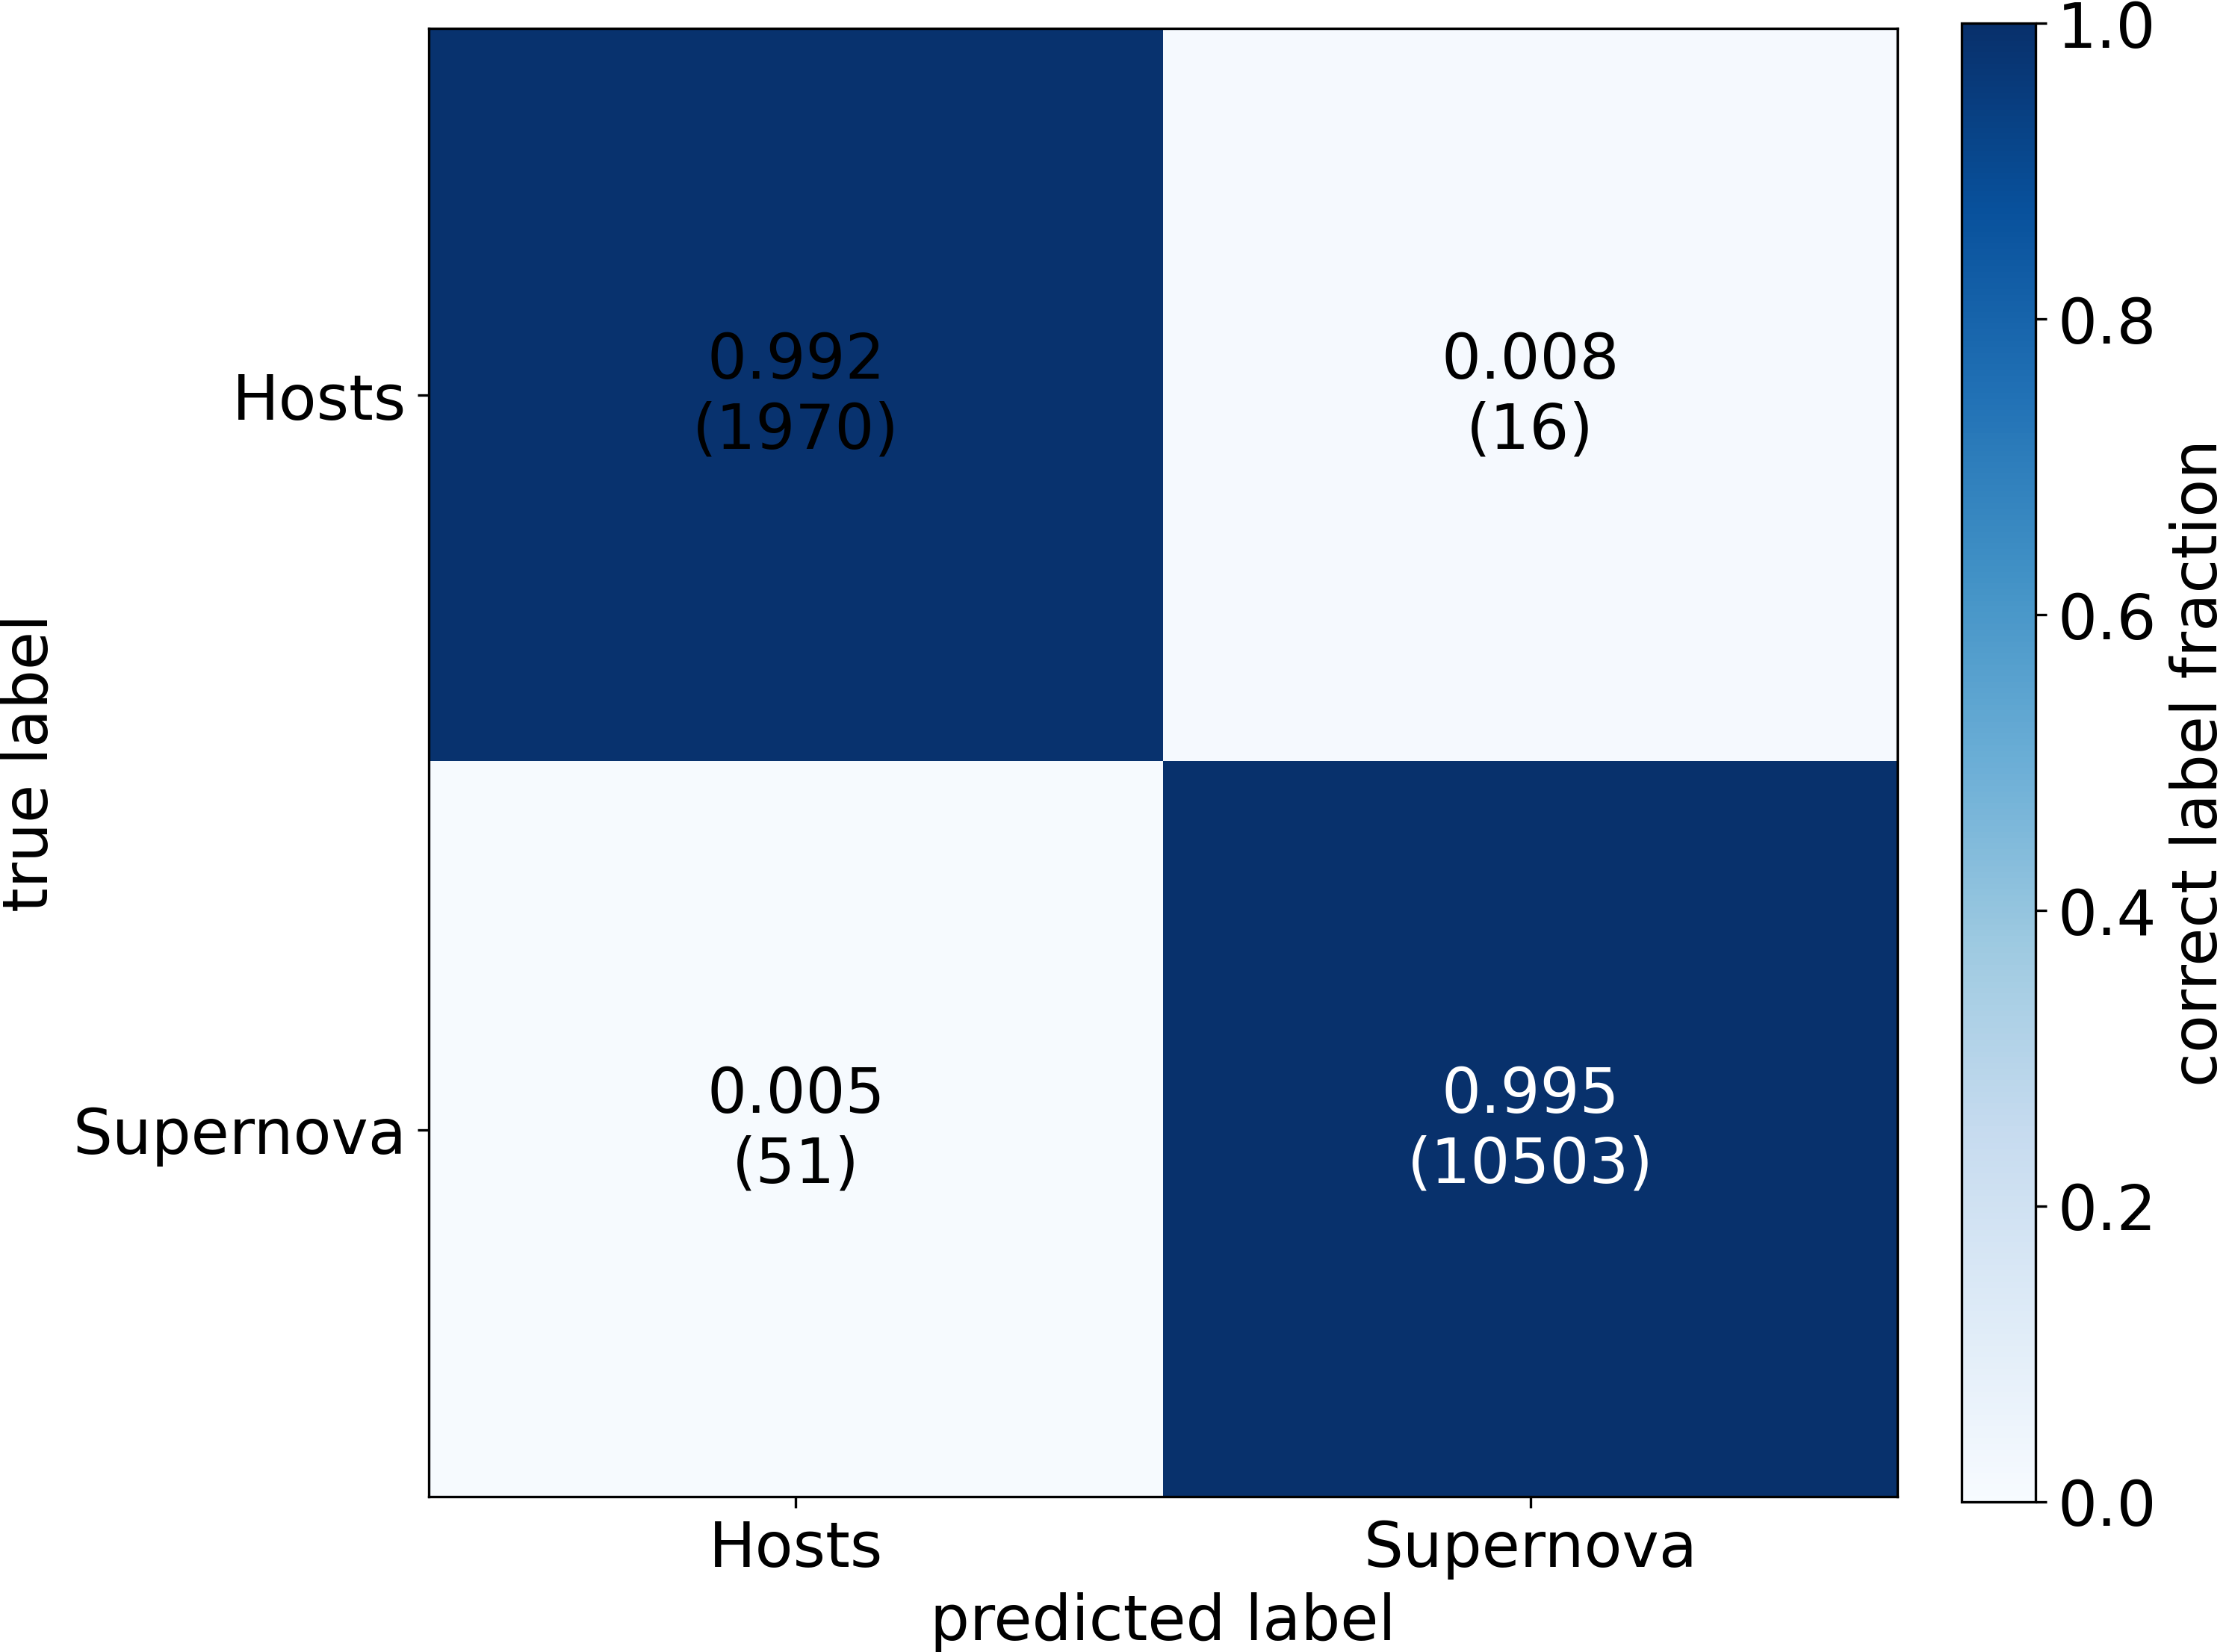
\includegraphics[height=4.2cm]{figures/v2_real/vit_model_V2cm9999_binary_e26.png}
    \caption{Spectral ViT V2 Binary Diagnostics: ROC Curve (left) and Confusion Matrix (right) with a 99.99\% confidence
    cut \label{fig:cnn_qual}}
\end{figure}

